% Auriga theme
% find the most up-to-date version here: https://github.com/anishathalye/auriga

\documentclass[14pt,aspectratio=169]{beamer}
\usepackage{pgfpages}
\usepackage{fancyvrb}
\usepackage{tikz}
\usepackage{tikz-qtree}

\usepackage{pgfplots}

\usepackage{booktabs}
\usepackage[normalem]{ulem}


\usetheme{auriga}
\usecolortheme{auriga}
%\setbeamercolor{math text}{fg=blue}

\newcommand\blfootnote[1]{%
\begingroup
\renewcommand\thefootnote{}\footnote{#1}%
\addtocounter{footnote}{-1}%
\endgroup
}

%\setbeamertemplate{footline}[]
%\renewcommand\footnotemark{}

\setbeamertemplate{footline}[frame number]

% define some colors for a consistent theme across slides
\definecolor{red}{RGB}{181, 23, 0}
\definecolor{blue}{RGB}{0, 118, 186}
\definecolor{gray}{RGB}{146, 146, 146}
\definecolor{orange}{RGB}{255, 165, 0}
\definecolor{green}{RGB}{0, 128, 0}
% Create a slide for each section
\AtBeginSection[]{
  \begin{frame}
    \vfill
    \centering
    \begin{beamercolorbox}[sep=8pt,center,shadow=true,rounded=true]{title}
      \usebeamerfont{title}\insertsectionhead\par%
    \end{beamercolorbox}
    \vfill
  \end{frame}
}

\title{Do we need \textcolor{blue}{Attention}?}

\author{Presented by Sasha Rush}

% \institute[shortinst]{}

\begin{document}

{
  % rather than use the frame options [noframenumbering,plain], we make the
  % color match, so that the indicated page numbers match PDF page numbers
  \setbeamercolor{page number in head/foot}{fg=background canvas.bg}
  \begin{frame}
    \titlepage
  \end{frame}
}

\begin{frame}[label=c]{}
    \textit{
    This talk is a survey of work done by:
}
    
    \begin{center}
    Albert Gu, Ankit Gupta, Tri Dao, Dan Fu, Shuangfei Zhai, Antono Orvieto, Michael Poli, Chris Re, Yuhon Li, Tianle Cai, Harsh Mehta, Jimmy Smith, Scott Linderman, Xuezhe Ma, Chunting Zhou, Xiang Kong, Bo Peng, Eric Alcaide, Anthony Quentin, Andrew Warrington, Yi Zhang, Stefano Massaroli, \\and many others
    \end{center}

\end{frame}

\section{Preface: Transformers and Attention}



% \begin{frame}[c]{}
%     \centering
%     \begin{figure}
%         \centering
%         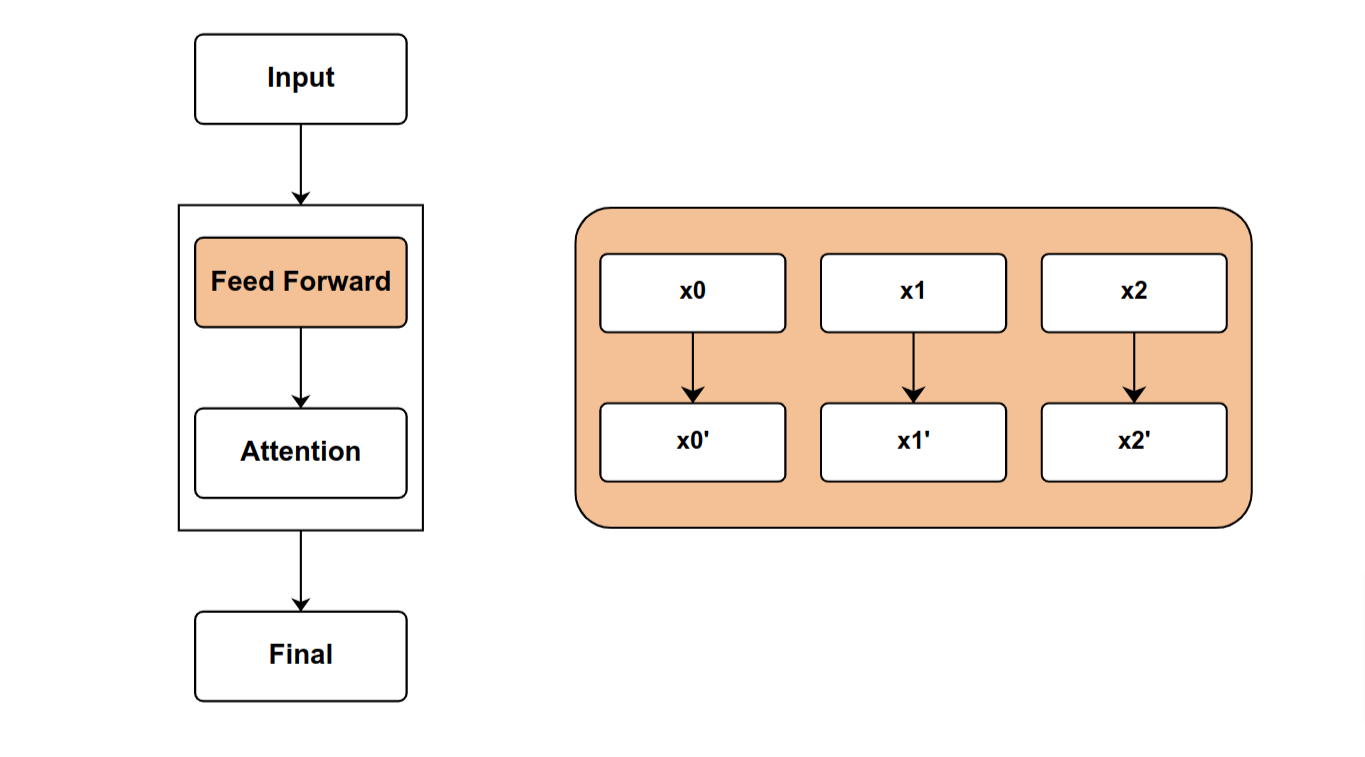
\includegraphics[height=0.9\textheight]{Figs/FeedForward.png}
%         \label{fig:my_label}
%     \end{figure}
% \end{frame}

\begin{frame}[c]{Transformers for Sequence Modeling}
    \centering
    \begin{columns}
    \begin{column}{0.3\textwidth}
        Repeated components 
        \vspace{0.5cm}
        
            \begin{itemize}
                \item Feed Forward

                \item Attention 
            \end{itemize}
    \end{column}        
    \begin{column}{0.7\textwidth}

    \begin{figure}
        \centering
        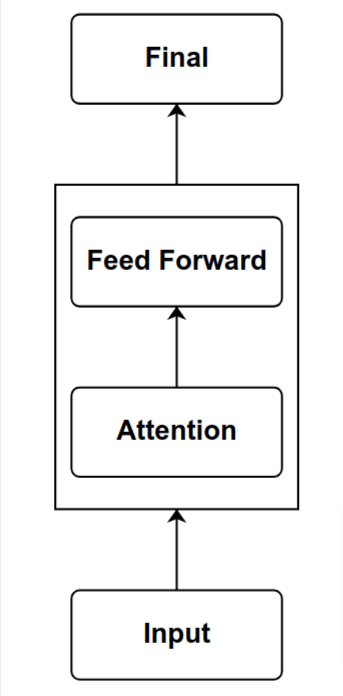
\includegraphics[height=0.8\textheight,  clip,trim={0.1cm 0.1cm 0.1cm 0.1cm}]{Figs/out.png}
        %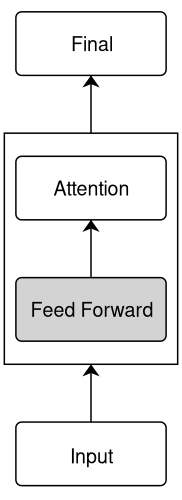
\includegraphics[height=0.8\textheight]{Figs/out2 (1).png} \label{fig:my_label}
    \end{figure}
    \end{column}
    \end{columns}        

\end{frame}

\begin{frame}{Feed Forward}
    \begin{itemize}
        \item Acts on each position independently. 
    \end{itemize}
    \begin{figure}
        \centering
        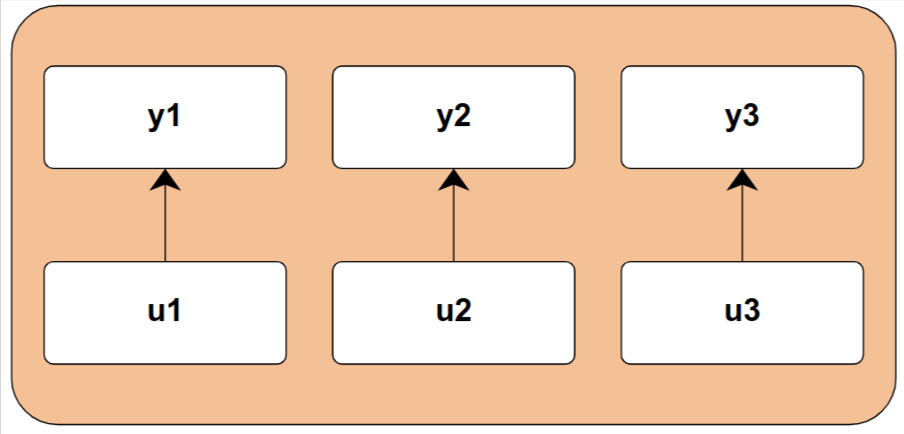
\includegraphics[height=0.5\textheight, clip,trim={0.1cm 0.1cm 0.1cm 0.1cm}]{Figs/out4.png}
    \end{figure}
\end{frame}

\begin{frame}[c]{Attention} 
    \begin{itemize}
        \item Fully connected interactions.
    \end{itemize}

    \centering
    \begin{figure}
        \centering
        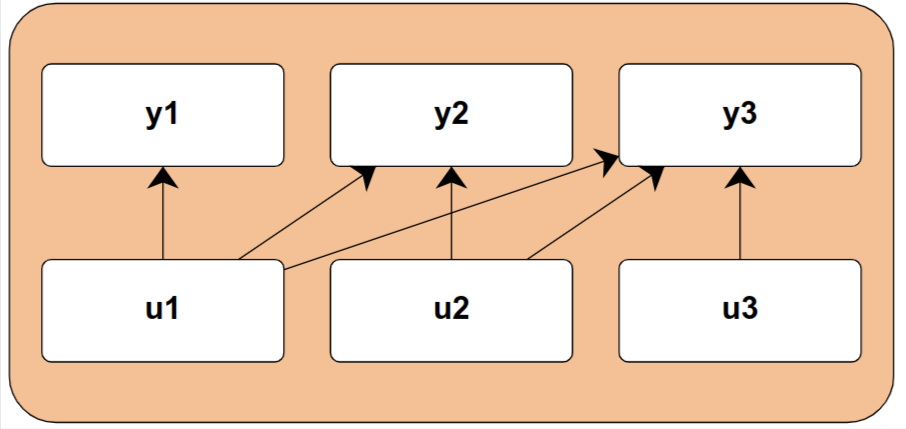
\includegraphics[height=0.5\textheight,  clip,trim={0.1cm 0.1cm 0.1cm 0.1cm}]{Figs/out5.png}
        \label{fig:my_label}
    \end{figure}    
\end{frame}


% \begin{frame}{Attention Matrix}
%         \centering
%     \begin{itemize}
%         \item Schematic of interactions at each layer (quadratic)
%     \end{itemize}

    
%     \begin{figure}
%         \centering
%         % 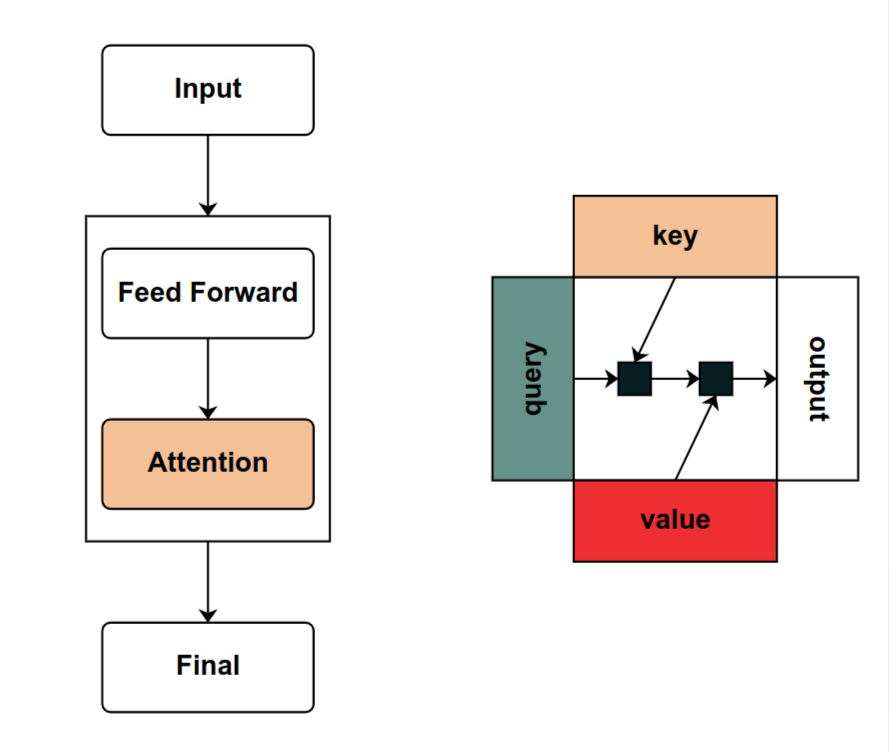
\includegraphics[height=0.7\textheight,clip,trim={14cm 3cm 0.5cm 3cm}]{Figs/Attention.png} \hspace{1cm} 
%         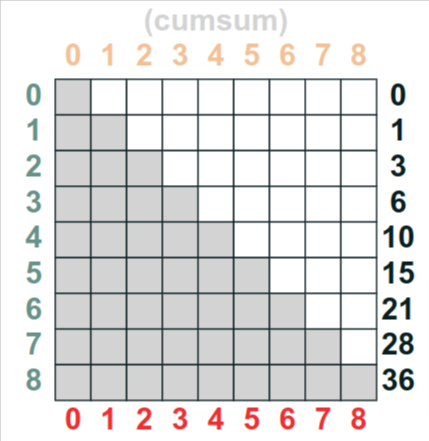
\includegraphics[height=0.7\textheight, clip, trim={1.5cm 1.3cm 0.1cm 0.1cm}]{Figs/Cumsum.png}
%         \label{fig:my_label}
%     \end{figure}
% \end{frame}


\begin{frame}[c]{Task: Language Generation}
    \centering
    Predict the next word.
    \vspace{1.5cm}
    

    \structure{Final:}  The dog walked to the \textcolor{red}{park}
    
    \vspace{1.5cm}
    
        \textcolor{blue}{Input:} The dog walked to the  \textcolor{red}{?}

\end{frame}

\begin{frame}[c]{Task: Long Range Arena (ListOps)}
    \centering
    Calculate the equation ($\uparrow$=max $\downarrow$=min)
    \vspace{1.5cm}

    
    \structure{Final:} [ $\uparrow$ 2 9 [ $\downarrow$ 4 7 ] 0 ] \textcolor{red}{9}
    
    \vspace{1.5cm}

    
    \textcolor{blue}{Input:}  [ $\uparrow$ 2 9 [ $\downarrow$ 4 7 ] 0 ] \textcolor{red}{?}
\end{frame}



\begin{frame}[c]{Attention Matrix}

    \centering

    \begin{center}
        All quadratic interactions possible.
    \end{center}
    
    \begin{figure}
        \centering
        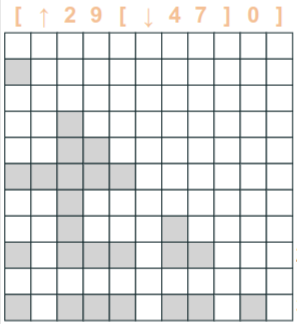
\includegraphics[height=0.6\textheight, clip,trim={0.1cm 0.1cm 0.1cm 0.1cm}]{Figs/Complex.png}
       \label{fig:my_label}
    \end{figure}
\end{frame}

\begin{frame}[c]{Attention for Realistic Examples}
    \centering
     \begin{center}
    Listops goes to 2,000 steps. This is 100.
    \end{center}

    \begin{figure}
        \centering
        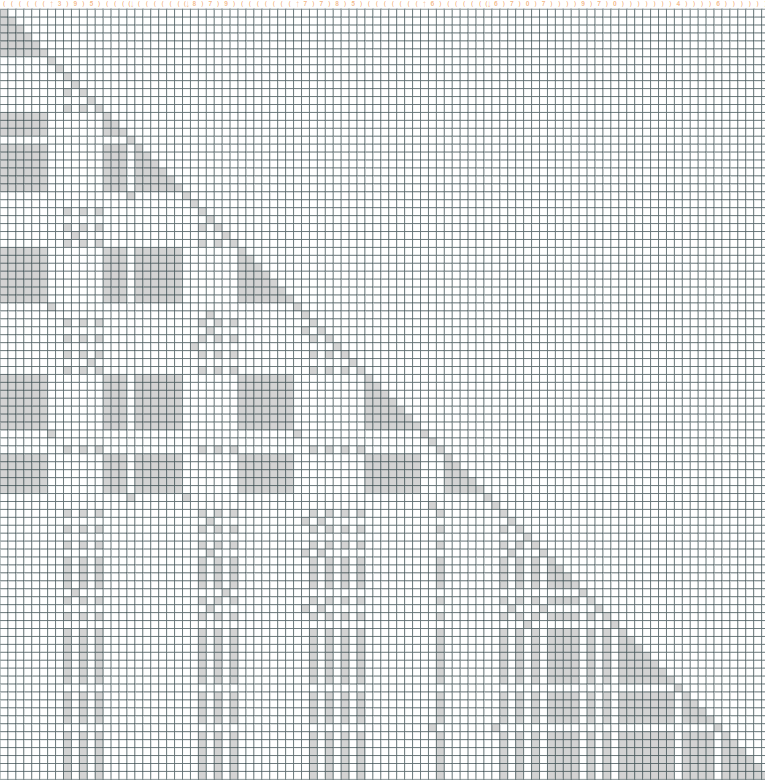
\includegraphics[height=0.6\textheight, clip,trim={0.1cm 0.1cm 0.1cm 0.1cm}]{Figs/big.png}
       \label{fig:my_label}
    \end{figure}
\end{frame}




    

\section{The Challenge}
\begin{frame}{Do we need \textcolor{blue}{Attention}?}
    \centering
    \only<2>{Or can we use something simpler...}
    \begin{figure}
        \centering
        
        \includegraphics<1>[height=0.6\textheight,clip,trim={0.1cm 0.1cm 0.1cm 0.1cm}]{Figs/Complex.png} 
        \includegraphics<2>[height=0.55\textheight,clip,trim={0.1cm 0.1cm 0.1cm 0.1cm}]{Figs/Allowed.png}
        
        
    \end{figure}
\end{frame}

\begin{frame}[label=current]{Proposition - One year ago}
    \begin{quote}
        On January 1, 2027, an \textcolor{blue}{Attention-based} model will be state-of-the-art in natural language processing.
    \end{quote}

    \begin{figure}
        \centering
        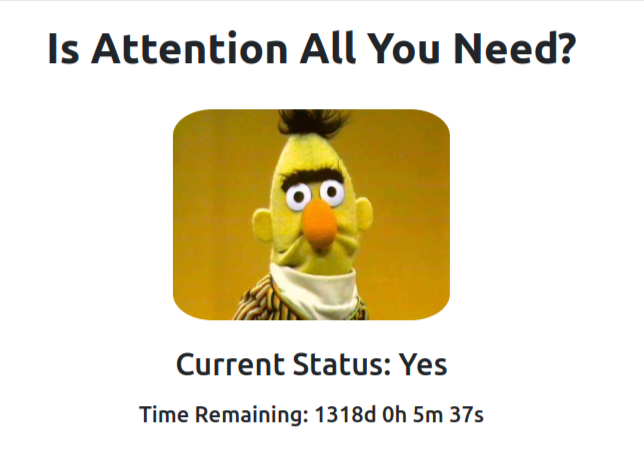
\includegraphics[width=0.7\linewidth,clip,  trim={0.1cm 0.1cm 0.1cm 0.1cm}]{Figs/Is-Attention-All-You-Need-.png}
        \label{fig:my_label}
    \end{figure}

\end{frame}


\begin{frame}[c, label=current]{}
    \begin{figure}
        \centering
    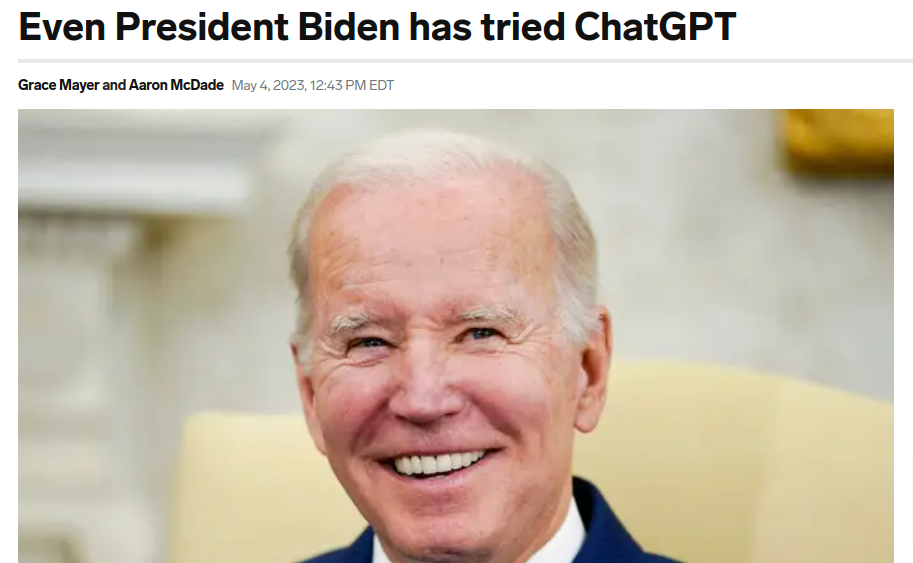
\includegraphics[width=0.8\linewidth]{Figs/Biden.png}
        \label{fig:my_label}
    \end{figure}
\end{frame}



\begin{frame}{Algorithmic Goal}
    GPT models are growing, but still limited by context length.
    \vspace{1cm}
    
    \begin{itemize}
        \item \textcolor{blue}{Training Speed} - Cost is quadratic in length
        \item \textcolor{blue}{Generation Speed} - Attention requires full lookback
    \end{itemize}
\end{frame}




\begin{frame}{Survey: Progress on Attention Alternatives}
    \begin{center}
        Recent research has made significant progress.
    \end{center}

    \begin{columns}
    \begin{column}{0.4\textwidth}
    \textit{S4}~\cite{gu2022parameterization}
    \textit{DSS}~\cite{gupta2022diagonal}
    \textit{GSS}~\cite{mehta2022long}
    \textit{S4D}~\cite{Gu2022-jz} 
    \textit{H3}~\cite{dao2022hungry}
    \textit{S5}~\cite{smith2022simplified}
    \textit{BiGS}~\cite{Wang2022-un}
    \end{column}
    \begin{column}{0.4\textwidth}      
    \textit{QRNN}~\cite{mccann2017learned}
    \textit{LRU}~\cite{Orvieto2023-an}
    \textit{RWKV}~\cite{Peng2023-yp}
    \textit{Mega}~\cite{ma2022mega}
    \textit{Hyena}~\cite{Poli2023-ag}
    \textit{SGConv}~\cite{Li2022-pn}
    \end{column}
    \end{columns}
    \pause

    
    \begin{center}
        \structure{Note:} Just one research direction.
        
    \end{center}


\end{frame}





\section{An RNN Revival}
 \begin{frame}{Discrete Time Sequence}

From \structure{scalar} sequence $u_{1}, \ldots, u_L$ to $y_1, \ldots, y_L$.

\begin{figure}
    \centering
    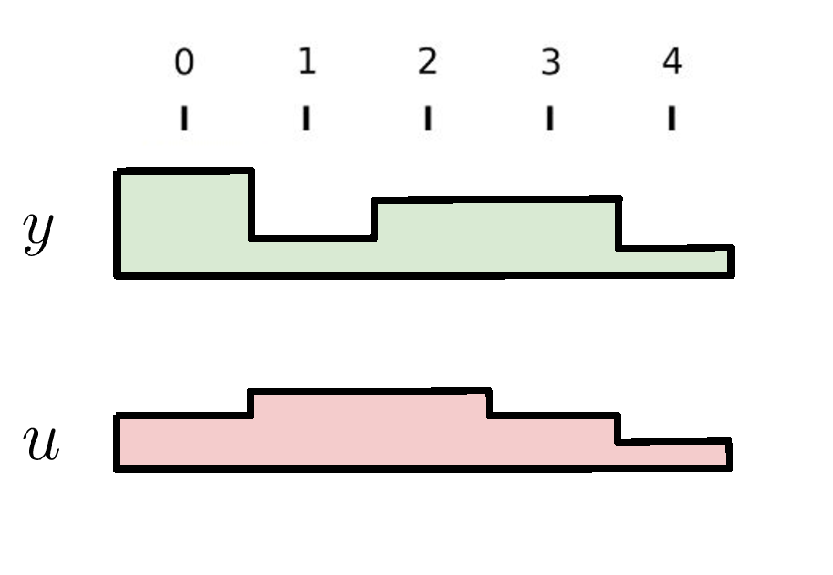
\includegraphics[width=0.5\textwidth]{Figs/SSMStart.pdf}
    \label{fig:my_label}
\end{figure}
\end{frame}


\begin{frame}{Review: RNN for Language Generation}
    \begin{columns}
    \begin{column}{0.5\textwidth}
        \centering
              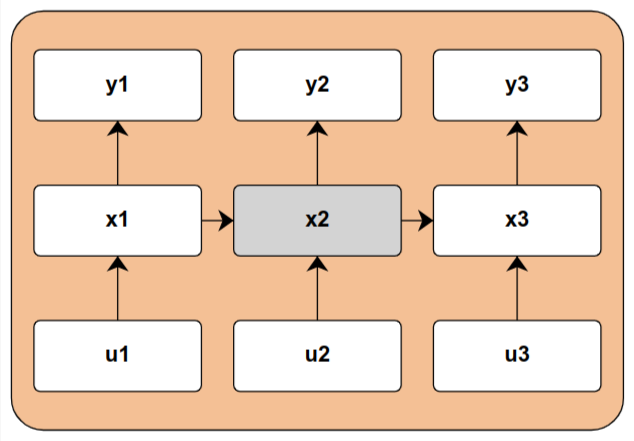
\includegraphics[width=.8\textwidth]{Figs/rnn.png}

    \end{column}
    \begin{column}{0.5\textwidth}

    \begin{align*}
    x_{k} &= \textcolor{red}{\sigma}(\textcolor{green}{\boldsymbol{\overline{A}}} x_{k-1} + \textcolor{blue}{\boldsymbol{\overline{B}}} u_k) \\ 
    y_k &= \phantom{\sigma (} \textcolor{orange}{\boldsymbol{\overline{C}}} x_{k \phantom{- 1}}
    \end{align*}
    \end{column}
    \end{columns}

\end{frame}

\begin{frame}{Review: RNN versus Attention}
    \begin{columns}
    \begin{column}{0.5\textwidth}
        \centering
        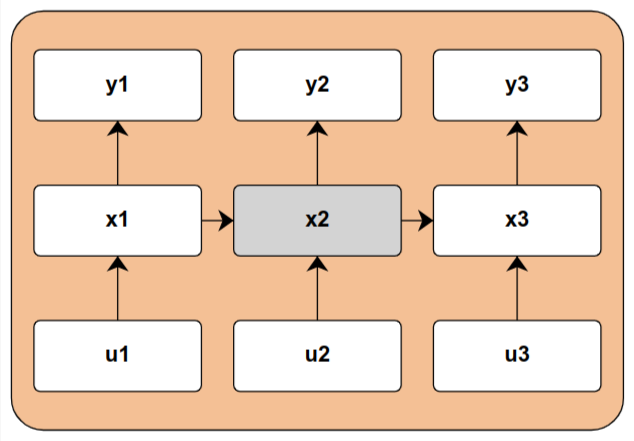
\includegraphics[width=.8\textwidth]{Figs/rnn.png}
    \end{column}
    \begin{column}{0.5\textwidth}
        \centering
  
        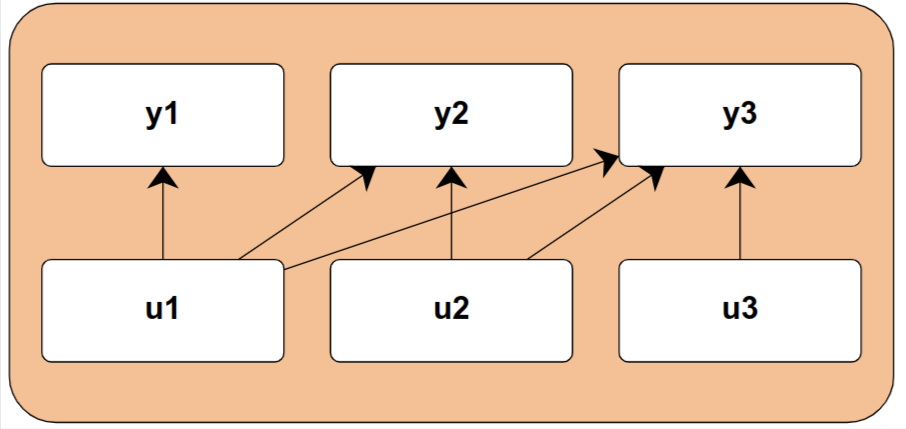
\includegraphics[width=0.8\textwidth]{Figs/out5.png}
    \end{column}
    \end{columns}
    \vspace{0.5cm}
    
\begin{itemize}
    \item \structure{Training Speed:} Slow (\textcolor{red}{Serial} bottleneck)
    \item \structure{Generation Speed:} Fast (constant-time per step)
    
\end{itemize}
\end{frame}


\begin{frame}{Didn't we try this RNN thing?  }

\begin{center}    
The last major RNN model in NLP - \textcolor{red}{ELMo}
\end{center}

\pause

    \begin{figure}
        \centering
        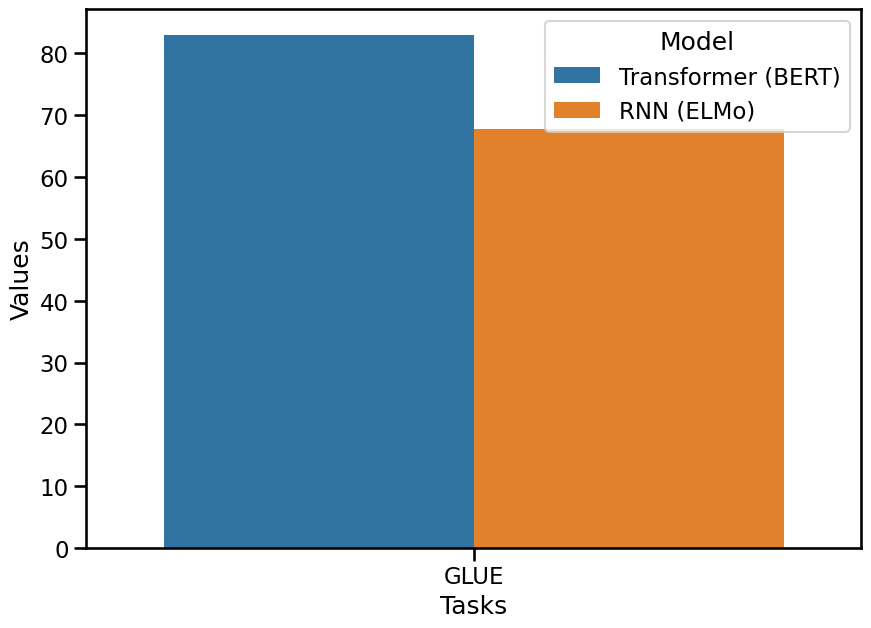
\includegraphics[width=0.5\textwidth]{Figs/GLUE.png}

        \label{fig:my_label}
    \end{figure}
\blfootnote{\cite{DBLP:conf/naacl/PetersNIGCLZ18, devlin2018bert}}
\end{frame}

\begin{frame}{RNN Revival: Two Differences}
\begin{columns}
    \begin{column}{0.5\textwidth}
        
    \begin{enumerate}
        \item Efficient Linear RNNs
        \item Effective Long-Range Parameterizations
    \end{enumerate}

    
    % Orthogonal RNN - Linear 
    % QRNN - > Linear RNN. $\bar{A}$ time-varying Linear non-homogenous. input depdendent 

    % A static over time. 
    % SISO - property. 
    % Orthogonal - > 
    
    \end{column}
    \begin{column}{0.5\textwidth}
\centering
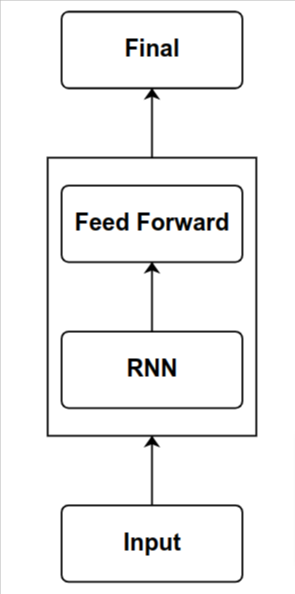
\includegraphics[width=0.4\textwidth, clip,trim={0.1cm 0.1cm 0.1cm 0.1cm}]{Figs/out-rnn.png}
    \end{column}

\end{columns}
\end{frame}



\begin{frame}{Component 1: \textcolor{blue}{Linear} RNN}

    \begin{align*}
    x_{k} &= \textcolor{green}{\boldsymbol{\overline{A}}} \textcolor{black}{\boldsymbol{x}_{k-1}} + \textcolor{blue}{\boldsymbol{\overline{B}}} \textcolor{black}{u_k} \\ 
    y_k &=  \textcolor{orange}{\boldsymbol{\overline{C}}} x_{k \phantom{- 1}}
    \end{align*}
    \pause
    \begin{figure}
        \centering
        
\includegraphics[width=0.6\textwidth]{Figs/ssm.png}
        \label{fig:my_label}
    \end{figure}
\end{frame}

\begin{frame}{Expansion Of Terms}
\vspace{-0.5cm}
    \begin{align*}
    y_k =  \textcolor{orange}{\boldsymbol{\overline{C}}} x_{k \phantom{- 1}} \ 
    x_{k} = \textcolor{green}{\boldsymbol{\overline{A}}} \textcolor{black}{\boldsymbol{x}_{k-1}} + \textcolor{blue}{\boldsymbol{\overline{B}}} \textcolor{black}{u_k} \ 
    \end{align*}
    \pause 
    \vspace{-2cm}
\begin{figure}
    \centering
    \only<2>{\[y_1\]}\only<3>{\[y_2\]} \only<4->{\[y_3\]}
    \includegraphics<2>[height=0.12\textwidth]{Figs/ssmrec0}
    
    \includegraphics<3>[height=0.12\textwidth]{Figs/ssmrec1}
    
     \includegraphics<4->[height=0.1\textwidth]{Figs/ssmrec}
    \label{fig:my_label}
\end{figure}
\vspace{-0.5cm}

\pause\pause\pause
\begin{align*}
\overline{K} &= (\textcolor{orange}{\boldsymbol{\overline{C}}}\textcolor{blue}{\boldsymbol{\overline{B}}}, \textcolor{orange}{\boldsymbol{\overline{C}}}\textcolor{green}{\boldsymbol{\overline{A}}}\textcolor{blue}{\boldsymbol{\overline{B}}}, \dots, \textcolor{orange}{\boldsymbol{\overline{C}}}\textcolor{green}{\boldsymbol{\overline{A}}^{L-1}}\textcolor{blue}{\boldsymbol{\overline{B}}})
\end{align*}
\end{frame}

\begin{frame}{Convolutional Form}

    \begin{align*}
    y_k =  \textcolor{orange}{\boldsymbol{\overline{C}}} x_{k \phantom{- 1}} \ 
    x_{k} = \textcolor{green}{\boldsymbol{\overline{A}}} \textcolor{black}{\boldsymbol{x}_{k-1}} + \textcolor{blue}{\boldsymbol{\overline{B}}} \textcolor{black}{u_k} \ 
    \end{align*}



\begin{align*}
\overline{K} &= (\textcolor{orange}{\boldsymbol{\overline{C}}}\textcolor{blue}{\boldsymbol{\overline{B}}}, \textcolor{orange}{\boldsymbol{\overline{C}}}\textcolor{green}{\boldsymbol{\overline{A}}}\textcolor{blue}{\boldsymbol{\overline{B}}}, \dots, \textcolor{orange}{\boldsymbol{\overline{C}}}\textcolor{green}{\boldsymbol{\overline{A}}^{L-1}}\textcolor{blue}{\boldsymbol{\overline{B}}}) \\
y &= \text{conv1d}(\overline{K}_L \ldots \overline{K}_1, u_1 \ldots u_L)
\end{align*}



% Intuition: 
% \pause
% $$y_1 = \boldsymbol{\overline{C}} \boldsymbol{\overline{B}} u_1$$ 
% \pause
% $$y_2 = \boldsymbol{\overline{C}} \boldsymbol{\overline{A}} \boldsymbol{\overline{B}} u_1 + \boldsymbol{\overline{C}} \boldsymbol{\overline{B}} u_2 = \boldsymbol{\overline{C}} (\boldsymbol{\overline{A}} \boldsymbol{\overline{B}} u_1 + \boldsymbol{\overline{B}} u_2) = \boldsymbol{\overline{C}} (\boldsymbol{x}_1 + \boldsymbol{\overline{B}} u_2) $$
\end{frame}


\begin{frame}{Convolutional Form}
\begin{align*}
\overline{K} &= (\textcolor{black}{\boldsymbol{\overline{C}}}\textcolor{black}{\boldsymbol{\overline{B}}}, \textcolor{black}{\boldsymbol{\overline{C}}}\textcolor{black}{\boldsymbol{\overline{A}}}\textcolor{black}{\boldsymbol{\overline{B}}}, \dots, \textcolor{black}{\boldsymbol{\overline{C}}}\textcolor{black}{\boldsymbol{\overline{A}}^{L-1}}\textcolor{black}{\boldsymbol{\overline{B}}}) \\
\end{align*}
\begin{figure}
    \centering
    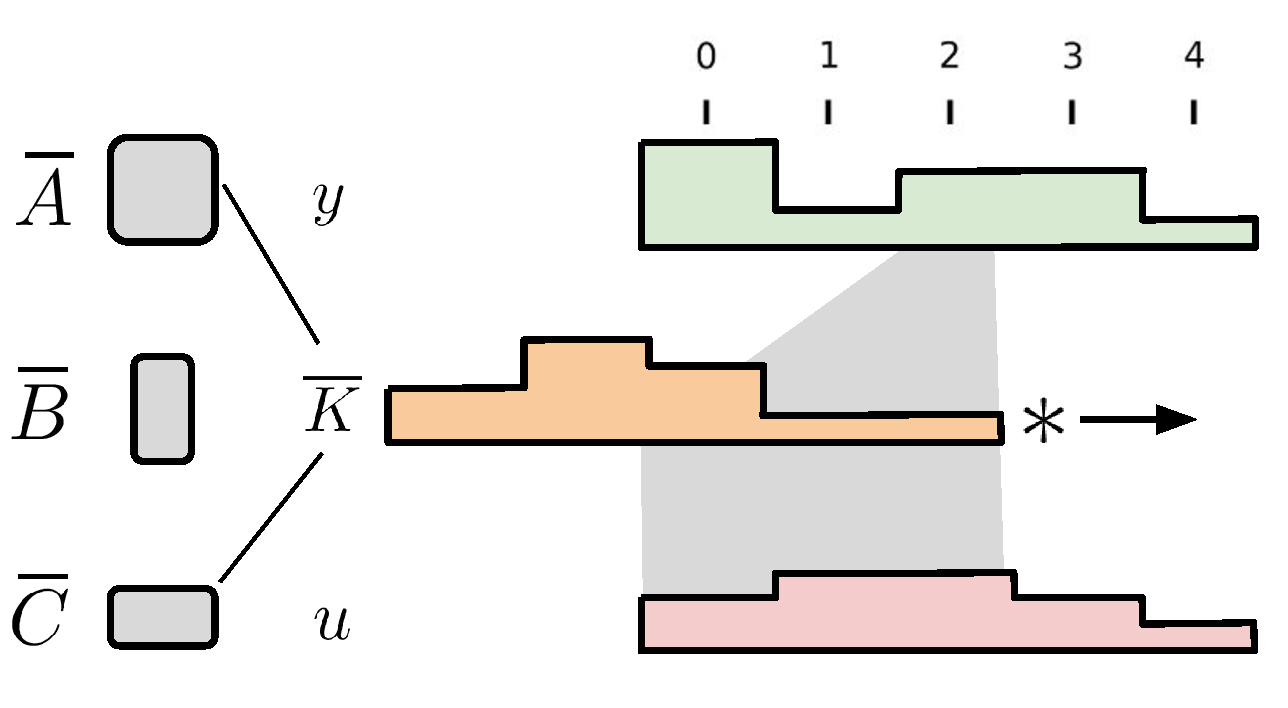
\includegraphics[width=0.6\textwidth]{Figs/SSM (1).pdf}
    \label{fig:my_label}
\end{figure}
\end{frame}

\begin{frame}{Computation 1: FFT}
Compute convolution in Fourier space, 

\begin{align*}
&y = \boldsymbol{\overline{K}} \ast u
\end{align*}
\begin{itemize}
    \item $O(L \log L)$ for padded FFT of $K$ and $u$, mult, then iFFT
    \item Accelerators optimize this to different levels.
\end{itemize}
\end{frame}

\begin{frame}[c]{Computation 2: Associative Scan (S5)}


\begin{columns}
    \begin{column}{0.5\textwidth}
    Associative $e_1\bullet \ldots \bullet e_L$

    \begin{center}
    \Tree [.$\bullet$ [.$\bullet$ [.$\bullet$ $e_1$ ] [.$\bullet$ $e_2$ ] ] [.$\bullet$ [.$\bullet$ $e_3$ ] [.$\bullet$ $e_4$ ] ] ]
    \end{center}
    \end{column}
        
 \begin{column}{0.5\textwidth}
 \centering
 \[e_k = (\boldsymbol{E}_k, \boldsymbol{e}_k) = (\bar{\textcolor{green}{\boldsymbol{A}}}, \bar{\textcolor{blue}{\boldsymbol{B}}}u_k)\]
    \begin{figure}
        \centering
        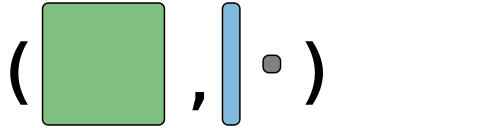
\includegraphics[height=0.1\textwidth,clip,trim={0cm 0cm 6cm 0cm}]{Figs/assoc.png}
        \label{fig:my_label}
    \end{figure}
    \[e_i \bullet e_j = (\boldsymbol{E}_i \boldsymbol{E}_j, \boldsymbol{E}_j \boldsymbol{e}_i + \boldsymbol{e}_j ) \]
    \begin{figure}
        \centering
        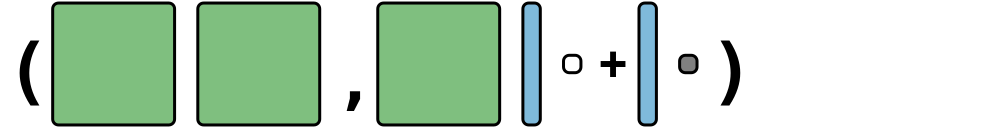
\includegraphics[height=0.1\textwidth,clip,trim={0cm 0cm 6cm 0cm}]{Figs/assoc2.png}
    \end{figure}
        
    \end{column}
\end{columns}
    \blfootnote{\cite{Blelloch1990-yo,Martin2018-bq,smith2022simplified}}
\end{frame}
% \begin{frame}{Alternative Computation: Associative Scan \cite{smith2022simplified}}
   

% \end{frame}


% \begin{frame}{ Associative Scan: S5 }
%     Potential benefits versus FFT
%     \vspace{0.5cm}
    
%     \begin{itemize}
%         \item Compute hidden states explicitly
%         \item Allows alternative RNN forms.
%         \item Faster on some architectures
%     \end{itemize}
% \end{frame}


\begin{frame}{Linear RNN Computational Profile}

    \begin{align*}
    x_{k} &= \textcolor{green}{\boldsymbol{\overline{A}}} \textcolor{black}{{x}_{k-1}} + \textcolor{blue}{\boldsymbol{\overline{B}}} \textcolor{black}{u_k} \\ 
    y_k &=  \textcolor{orange}{\boldsymbol{\overline{C}}} x_{k \phantom{- 1}}
    \end{align*}
\begin{itemize}
    \item \structure{Training Speed:} \sout{Weak} Strong (Parallelizable convolution)
    \item \structure{Generation Speed:} Strong (constant-time per step) \pause
    \item \structure{Accuracy:} Extremely \textcolor{red}{Poor...} Barely learns.
\end{itemize}
\end{frame}

\begin{frame}{Interactions}
    \begin{center}
        Routing here must be static and regular (conv). 
    \end{center}
    \begin{figure}
        \centering
        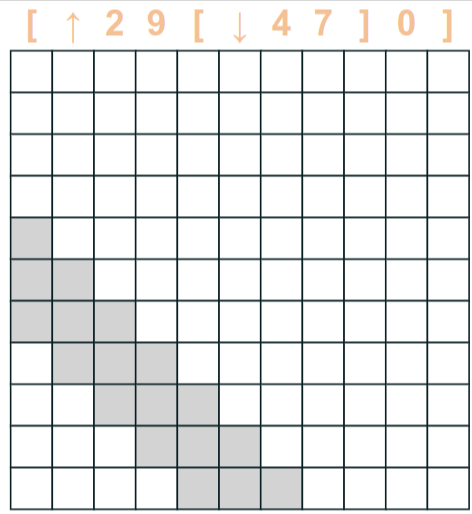
\includegraphics[height=0.45\textheight,clip,trim={0.1cm 0.1cm 0.1cm 0.1cm}]{Figs/Allowed.png}
        \vspace{0.5cm}
        
        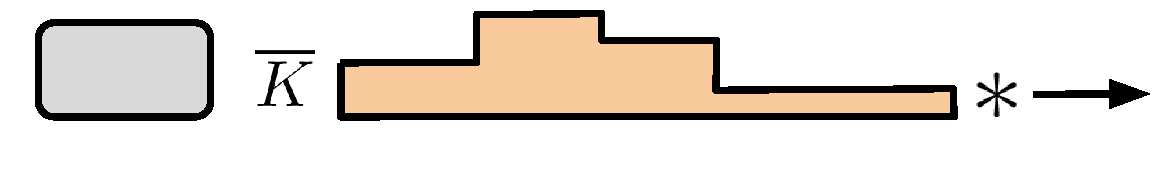
\includegraphics[width=0.5\textwidth]{Figs/SGParam.pdf}
        \label{fig:my_label}
    \end{figure}
\end{frame}




\begin{frame}{Component 2:  Model Parameterization}

Linear RNN behavior highly dependent on $\boldsymbol{\overline{A}}$

\begin{align*}
\overline{K} &= (\textcolor{orange}{\boldsymbol{\overline{C}}}\textcolor{blue}{\boldsymbol{\overline{B}}}, \textcolor{orange}{\boldsymbol{\overline{C}}}\textcolor{green}{\boldsymbol{\overline{A}}}\textcolor{blue}{\boldsymbol{\overline{B}}}, \dots, \textcolor{orange}{\boldsymbol{\overline{C}}}\textcolor{green}{\boldsymbol{\overline{A}}^{L-1}}\textcolor{blue}{\boldsymbol{\overline{B}}})
\end{align*}
\vspace{0.5cm}

Choice of $\boldsymbol{\overline{A}}$ is critical: stable and informative.
\end{frame}


\begin{frame}{Mathematical Model: State Space Model (SSM) }

A SSM is a continuous-time, differential equation.
\begin{align*}
    x'(t) &= \boldsymbol{A}x(t) + \boldsymbol{B}u(t) \\  
    y(t) &= \boldsymbol{C}x(t).
\end{align*}

Used to explore Linear RNN parameterization.
\end{frame}

\begin{frame}{Hidden State Form~\cite{gu2020hippo}}
  \textcolor{red}{Summarize} history in vector $x$ with \textcolor{blue}{Legendre} coefficients 
    \begin{figure}
    \centering
    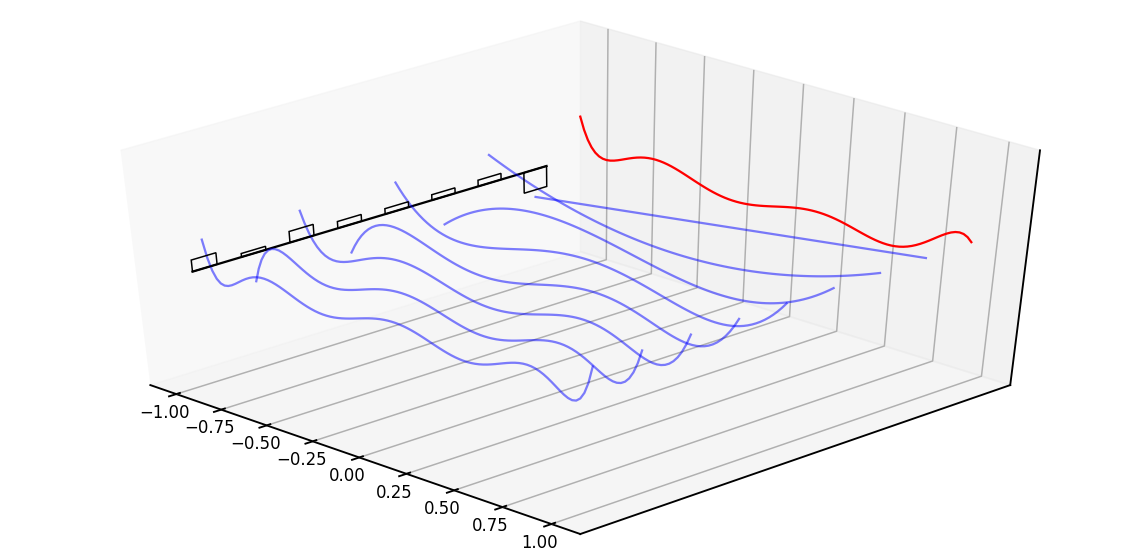
\includegraphics[width=0.7\textwidth]{Figs/hippo.png}
    \end{figure}
\end{frame}

\begin{frame}{Choice of Parameters~\cite{gu2020hippo}}
    Intuition: Hidden state vector $\textcolor{blue}{x}$ should \textcolor{red}{summarize} past $u$. 

\begin{figure}
    \centering
    \includegraphics<1>[width=\textwidth]{Figs/frame_10_delay-0.1s.png}
    \includegraphics<2>[width=\textwidth]{Figs/frame_20_delay-0.1s.png}
    \includegraphics<3>[width=\textwidth]{Figs/frame_30_delay-0.1s.png}
    \includegraphics<4>[width=1\textwidth]{Figs/frame_40_delay-0.1s.png}
    \includegraphics<5>[width=1\textwidth]{Figs/frame_50_delay-0.1s.png}
\end{figure}

\end{frame}



% \begin{frame}{Practical Consequence: HiPPO~\cite{gu2020hippo}}
%     Motivates an initialization of the (discrete-time) kernel $\bar{K}$.
    
%     \begin{figure}
%         \centering
%         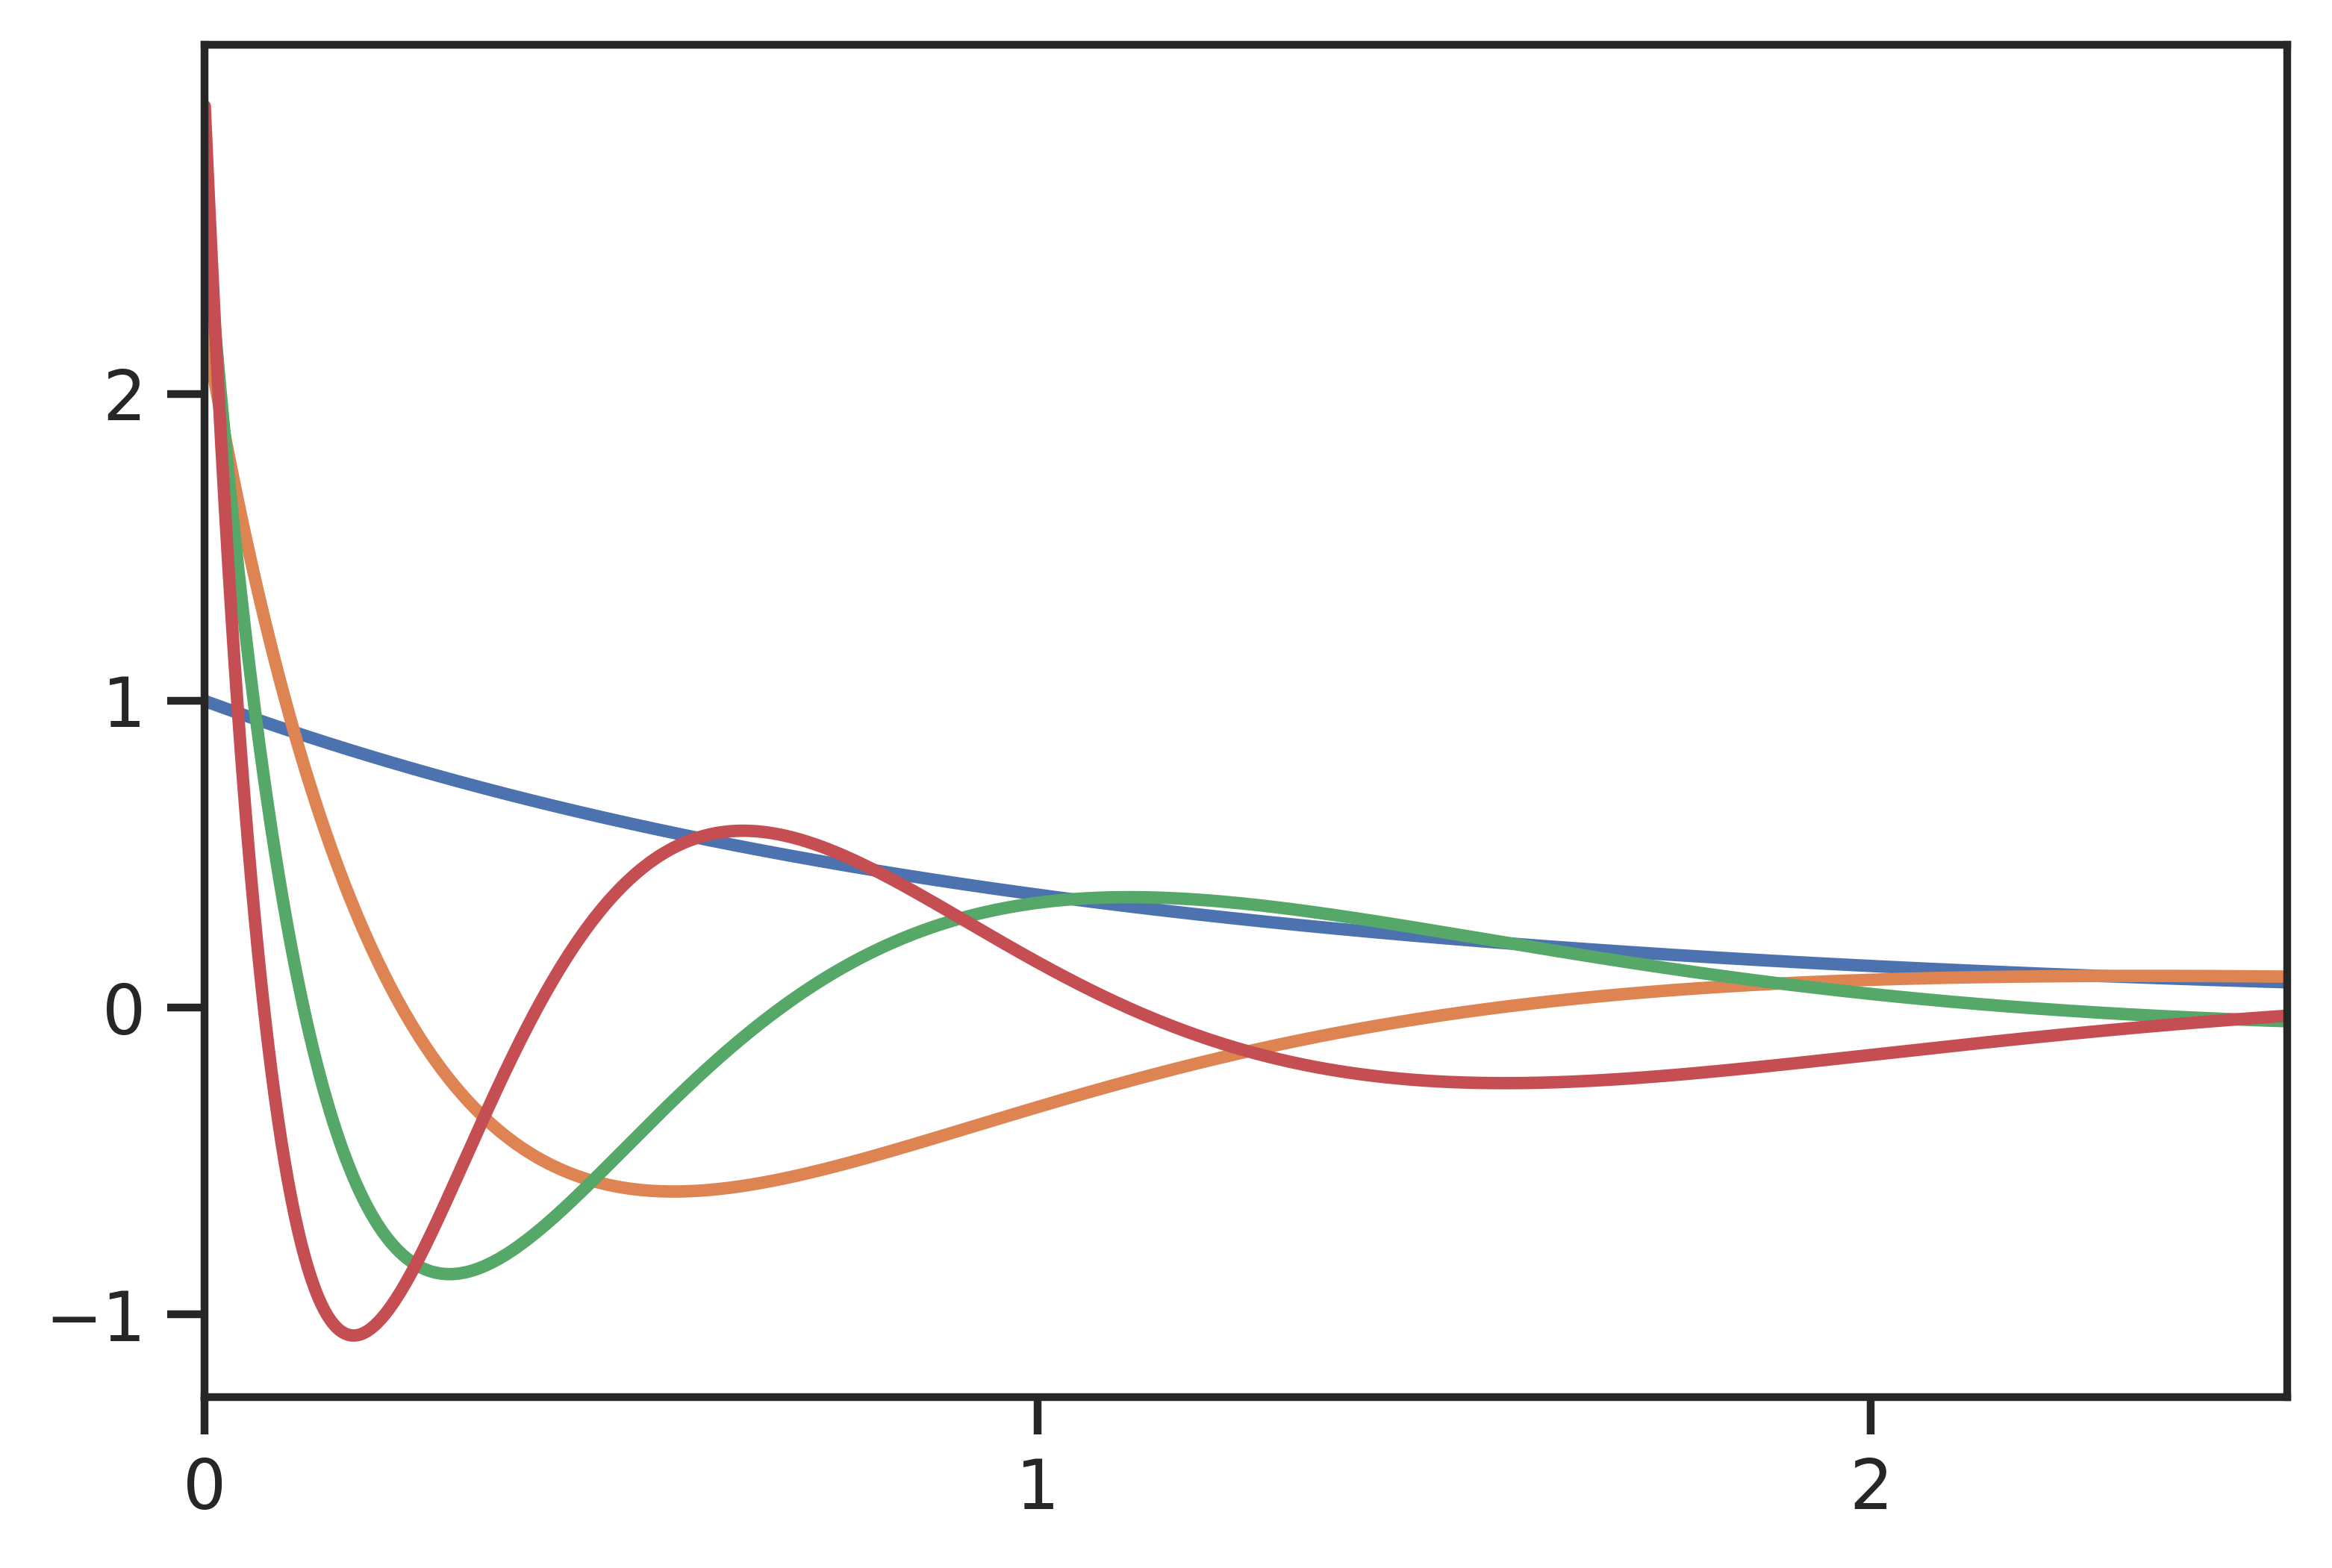
\includegraphics[width=0.5\textwidth]{Figs/hippo_kernel.png}
        
%         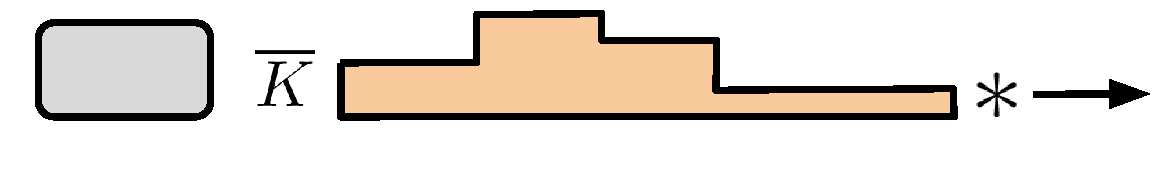
\includegraphics[width=0.5\textwidth]{Figs/SGParam.pdf}
%         \label{fig:enter-label}
%     \end{figure}
% \end{frame}

% \begin{frame}{S4 \cite{gu2022parameterization} }

% Learn parameters of SSM, convert to linear RNN parameters 

% $$\boldsymbol{\overline{A}}, \boldsymbol{\overline{B}}, \boldsymbol{\overline{C}}  = \text{discretize}(\boldsymbol{A}, \boldsymbol{B}, \boldsymbol{C}, \Delta )$$

%     \begin{figure}
%         \centering
%         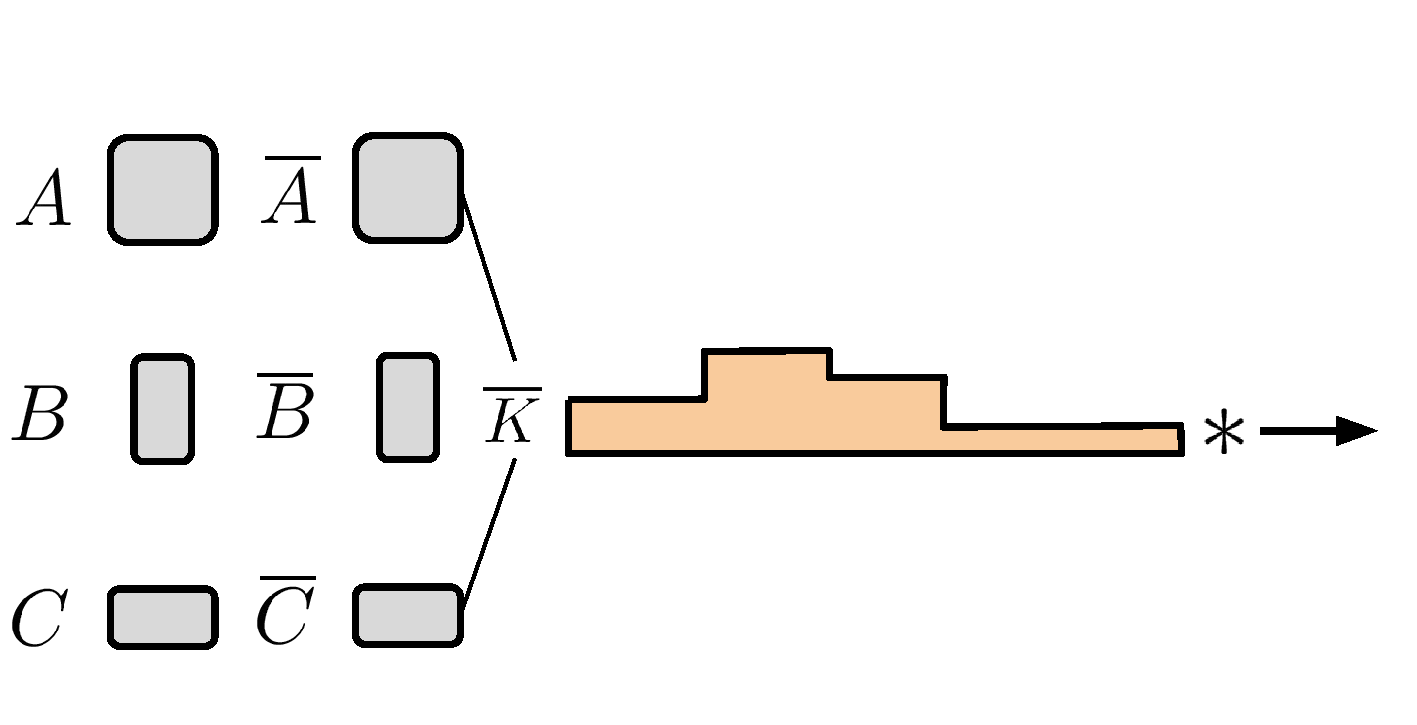
\includegraphics[width=0.6\textwidth]{Figs/SSMParam.pdf}
%         \caption{}
%         \label{fig:my_label}
%     \end{figure}
% \pause
% \vspace{-2cm}

% Note: There are \textit{many more} important details here.
    
% \end{frame}


% \begin{frame}{Determining RNN Parameterization}
% \begin{itemize}
% \item \cite{gu2020hippo} develop \textit{HiPPO} Matrix for SSM $\boldsymbol{A}$   

% % \begin{scriptsize}
% % \begin{align*}  
% % \boldsymbol{A}_{nk}= -
% % \begin{cases} 
% % (2n+1)^{1/2}(2k+1)^{1/2} & \text{if } n > k \\ n+1 &\text{if } n=k \text{\ else\ } 0
% % \end{cases} 
% % \end{align*}
% % \end{scriptsize}

%     \item Approximates history through Legendre coefficients 
% \end{itemize}
% \begin{figure}
%     \centering
%     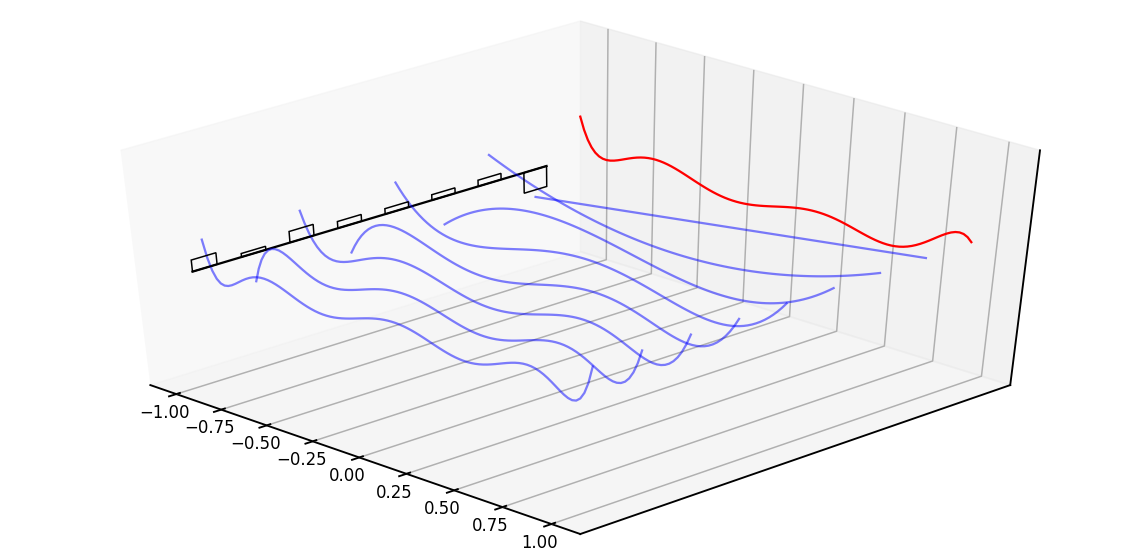
\includegraphics[width=0.7\textwidth]{Figs/hippo.png}
% \end{figure}
% \end{frame}

% \begin{frame}{Key Insight: Choice of $\boldsymbol{A}$ }

% \cite{gu2020hippo,gu2022parameterization}

% Show that HiPPO


% \end{frame}

\begin{frame}[c]{Results: ListOps \cite{gu2022parameterization}}
    \centering
        Example: [ $\uparrow$ 2 9 [ $\downarrow$ 4 7 ] 0 ] \textcolor{red}{9}
        
    \begin{figure}
        \centering

    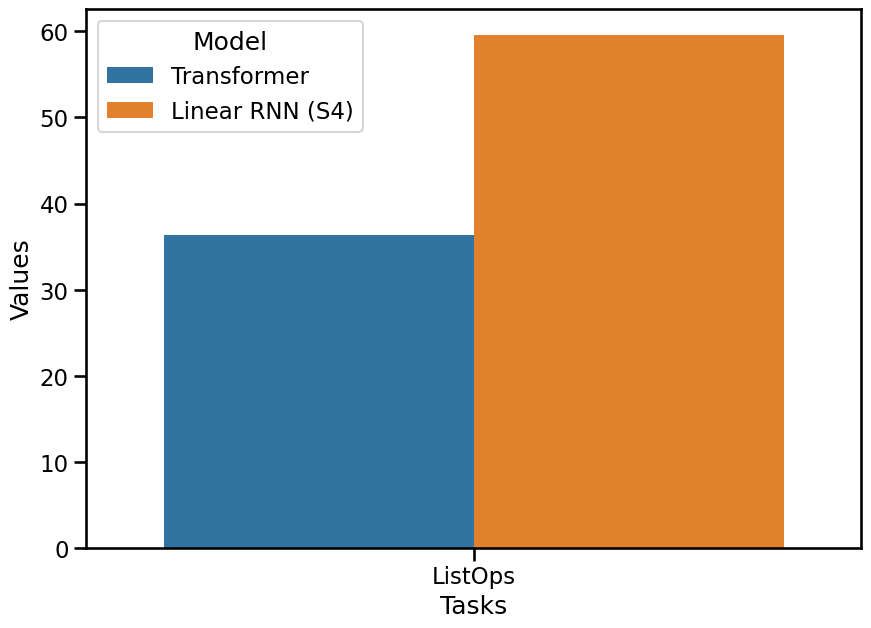
\includegraphics[height=0.6\textheight,clip,trim={0.1cm 0.1cm 0.1cm 0.1cm}]{Figs/listops-s4.png}
        \label{fig:my_label}
    \end{figure}
    Requires communication over 2,000  steps
    
\end{frame}


\begin{frame}[c]{Results: Long-Range Arena \cite{gu2022parameterization}}
    \centering
    \begin{figure}
        \centering
        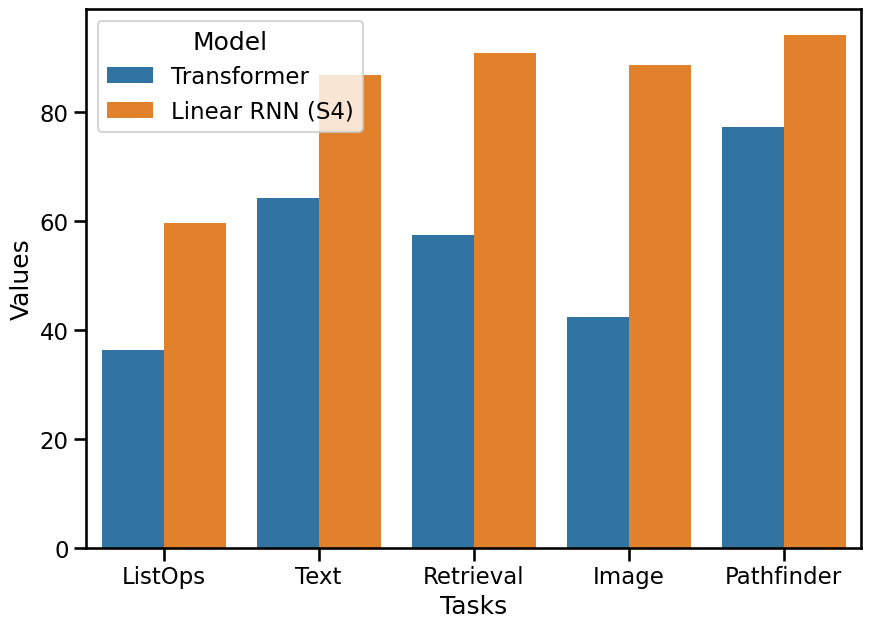
\includegraphics[height=0.8\textheight,clip,trim={0.1cm 0.1cm 0.1cm 0.1cm}]{Figs/lra-s4.png}
        \label{fig:my_label}
    \end{figure}
\end{frame}





% \begin{frame}{Computing with Static Kernels}
%     \structure{Final:} a b c $\Rightarrow$ d e f \textcolor{red}{d}

%     \begin{figure}
%         \centering
%         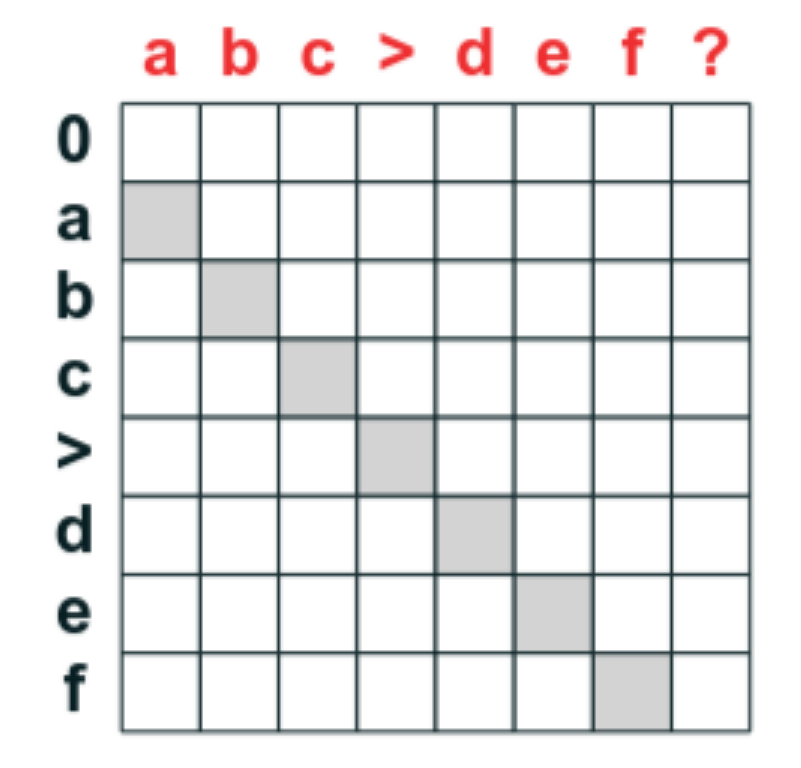
\includegraphics[height=0.5\textheight]{Figs/induct1.png}
%         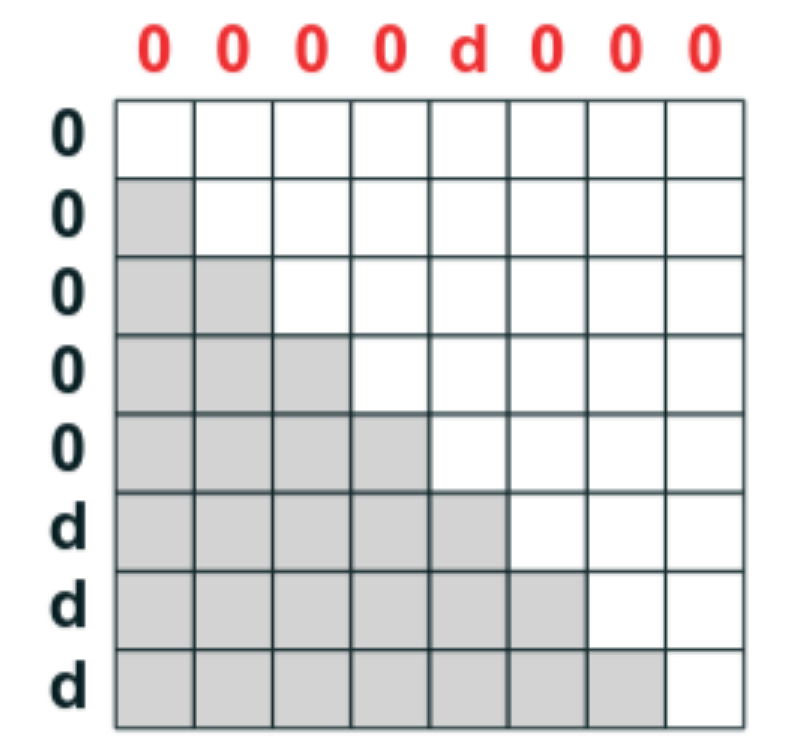
\includegraphics[height=0.5\textheight]{Figs/induct2.png}
%         \label{fig:my_label}
%     \end{figure}        
    
% \textcolor{blue}{Input:} a b c $\Rightarrow$ d e f \textcolor{red}{?}
 

% \end{frame}

\section{Are we GPT yet?}
 \begin{frame}{Applying Linear RNNs}
     \vspace{1cm}
     \begin{columns}
     \begin{column}{0.6\textwidth}         
     \begin{itemize}
         \item Speech~\cite{goel2022s}
         \item Video~\cite{Nguyen2022-qi}
         \item RL~\cite{Lu2023-ov}
         \item \textcolor{red}{NLP} 
     \end{itemize}
     \end{column}         
     \begin{column}{0.4\textwidth}         
    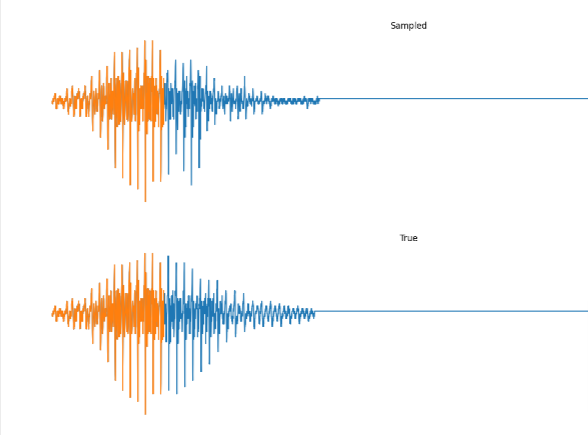
\includegraphics[width=0.9\textwidth, ,clip,trim={0.1cm 0.1cm 0.1cm 0.1cm}]{Figs/speech.png}
     \end{column}         

     \end{columns}    
\end{frame}

\begin{frame}{NLP Results}
    Two types of model
        \vspace{1cm}

    \begin{itemize}
        \item Bidirectional LM (BERT)
        \item Unidirectional LM (GPT)
    \end{itemize}
    \vspace{1cm}
    
    % Different architectures used, Some with partial attention
    
\end{frame}


\begin{frame}{Results: Bidirectional LM \cite{Wang2022-un}}
\begin{figure}
    \centering
    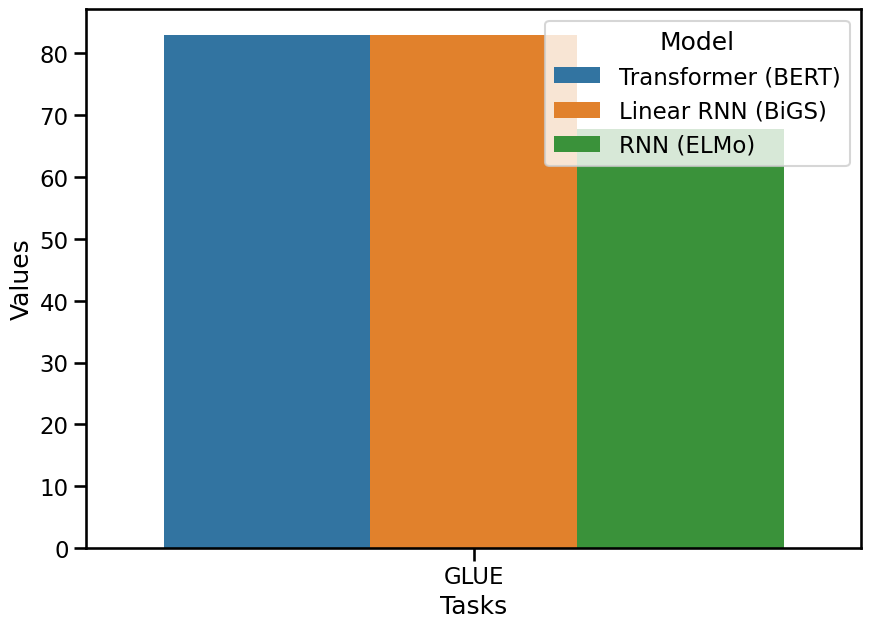
\includegraphics[height=0.6\textheight]{Figs/BiGS.png}
\end{figure}
\end{frame}


\begin{frame}{Analysis: Kernel Visualization $\boldsymbol{\bar{K}}$}

\begin{figure}
    \centering
    \includegraphics[width=\textwidth]{Figs/kernel1.png}
\end{figure}

\begin{itemize}
    \item Replaces Attention Matrix
    \item Single Kernel per layer 
\end{itemize}
\end{frame}

\begin{frame}{Analysis: All Kernels}
\begin{figure}
    \centering
    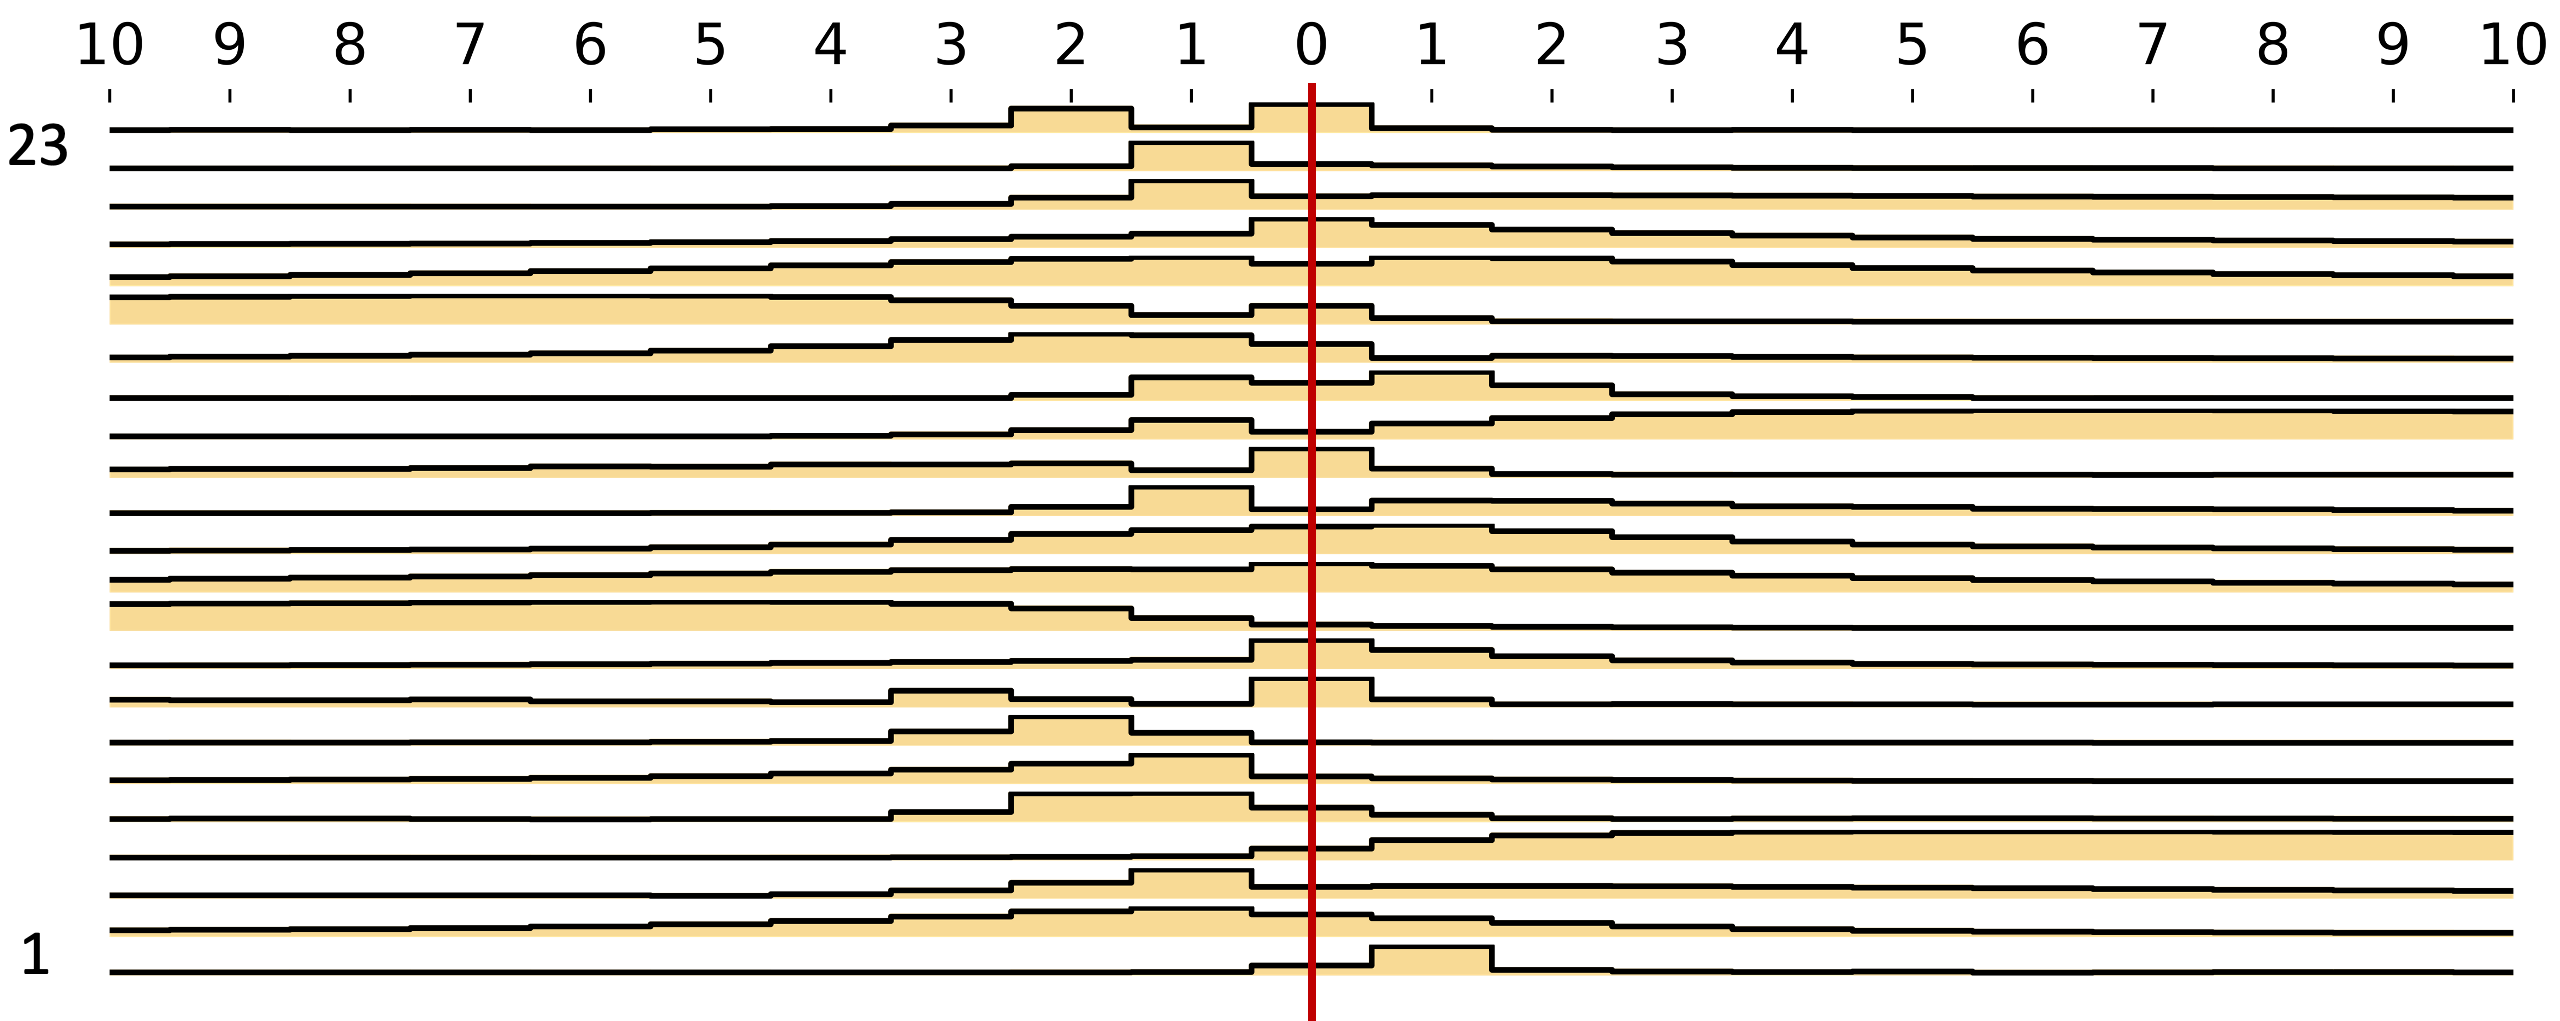
\includegraphics[height=0.6\textheight]{Figs/kernel2.png}
\end{figure}
\end{frame}

\begin{frame}{Analysis: Change in Kernels during Finetuning }

\centerline{Task: Long-Range Sentence Matching}
\begin{figure}
    \centering
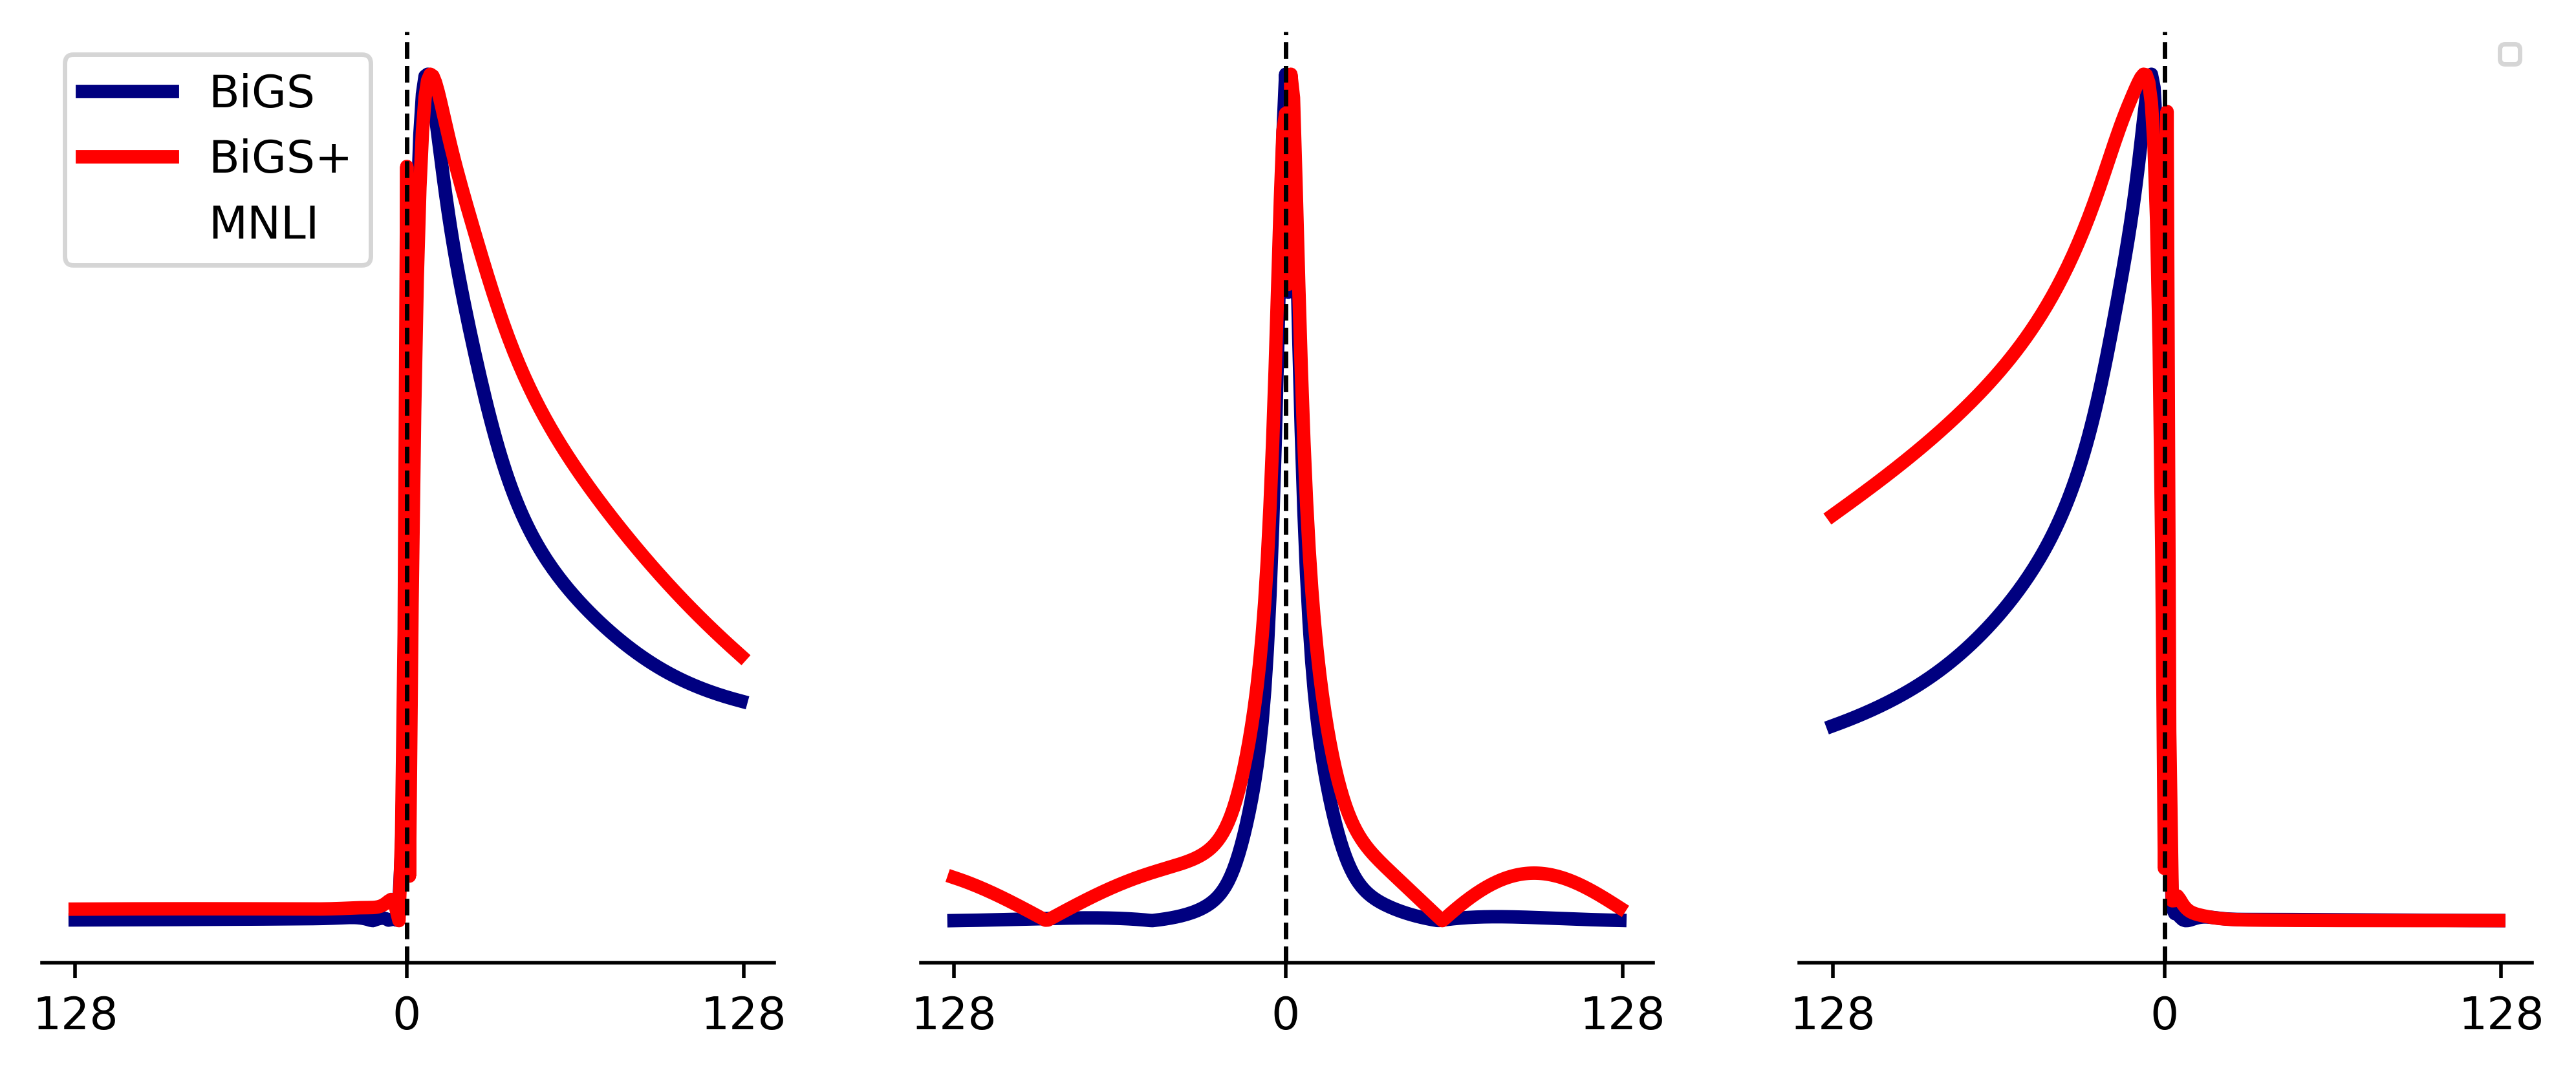
\includegraphics[width=0.8\textwidth]{Figs/comparison_results.png}
    \end{figure}
\end{frame}



\begin{frame}{Results: Unidirectional LM \cite{dao2022hungry}  $\downarrow$}
        \begin{figure}
        \centering
        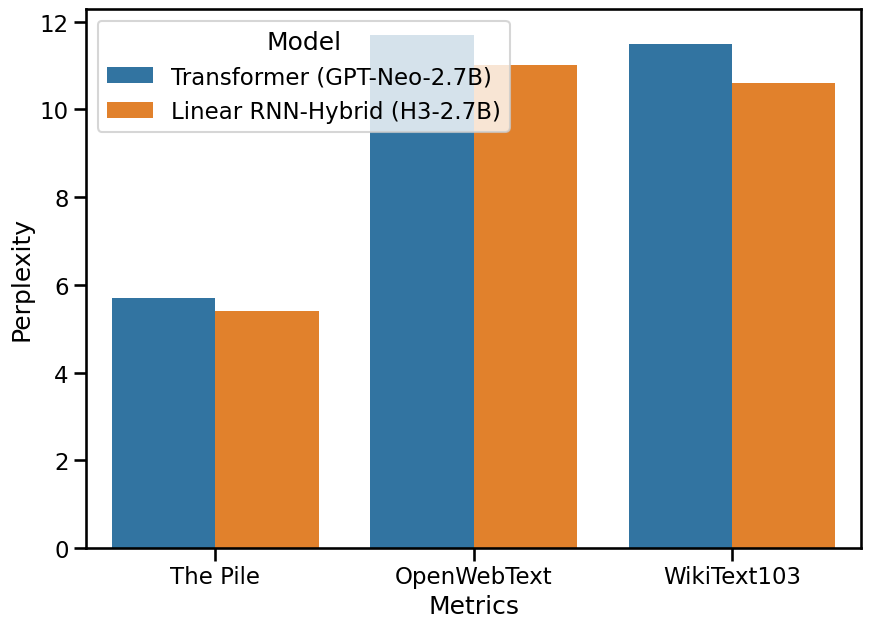
\includegraphics[width=0.7\textwidth]{Figs/H3.png}
        \caption{Caption}
        \label{fig:my_label}
    \end{figure}
\end{frame}

\begin{frame}
    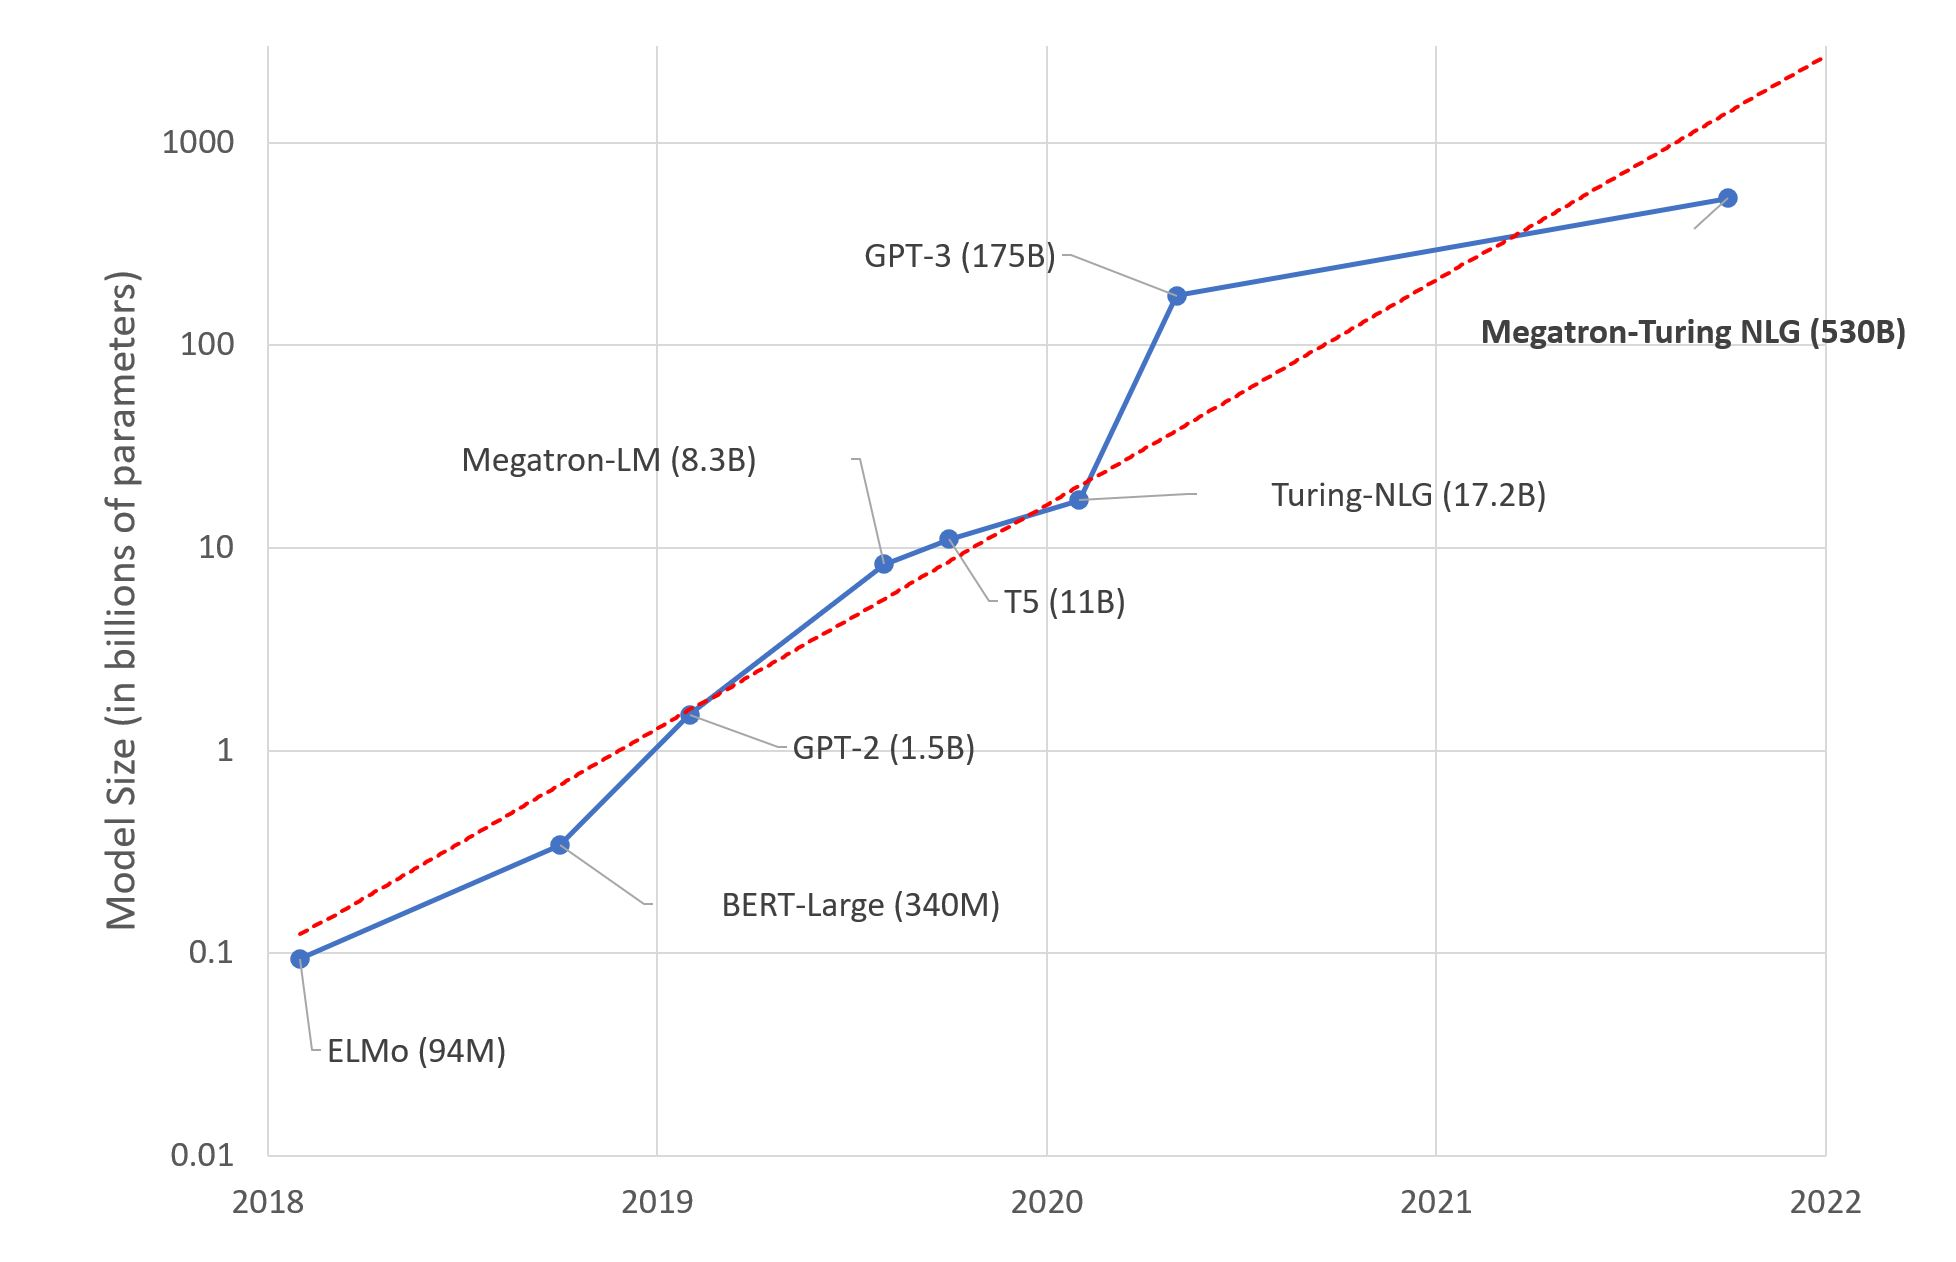
\includegraphics[ clip, height=\textheight]{Figs/ModelSize0.jpg}
\end{frame}

% \begin{frame}{Frame Title}
    
% \end{frame}

\section{Alternative Parameterizations}

\begin{frame}{Do we need the SSM?}
    \begin{figure}
        \centering
            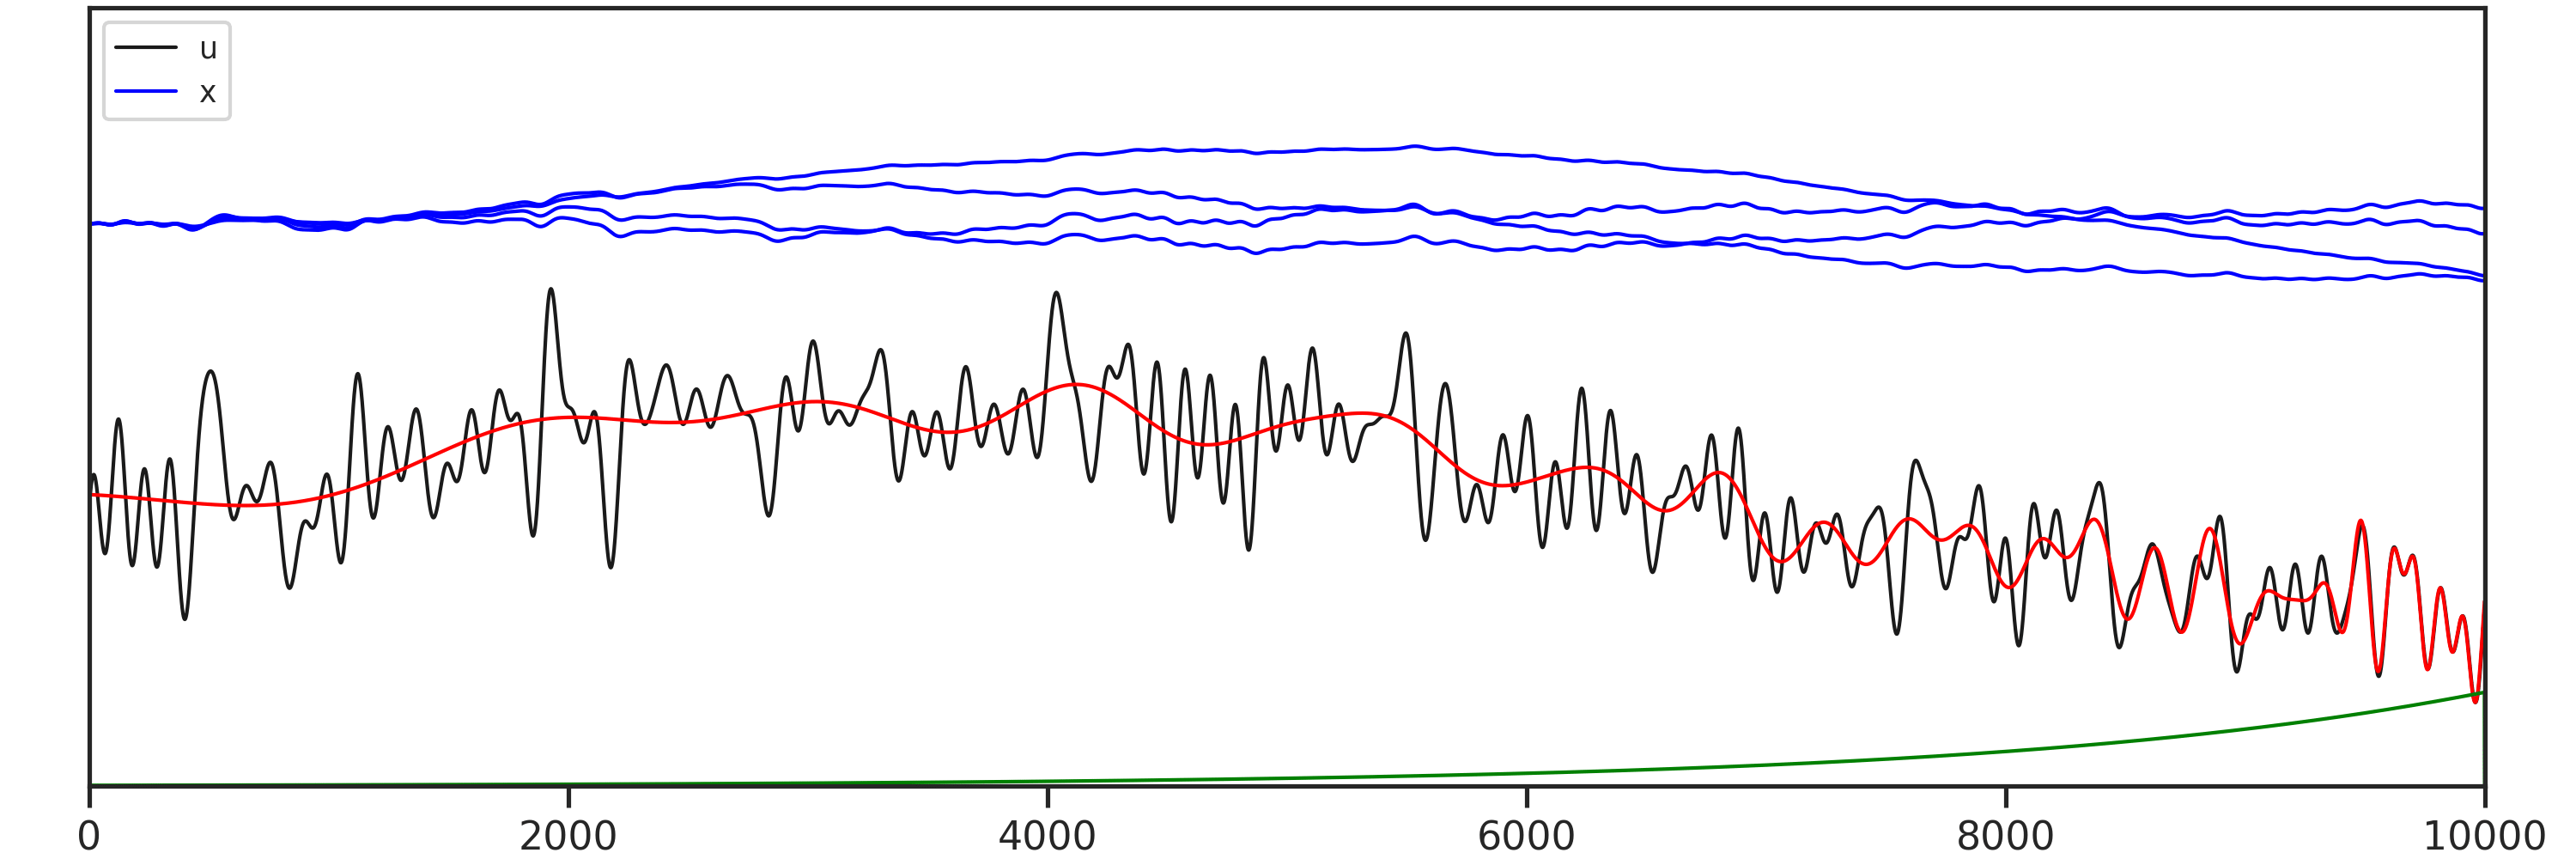
\includegraphics[width=1\textwidth]{Figs/frame_50_delay-0.1s.png}
    \end{figure}
\end{frame}

\begin{frame}{CNN Param: Decaying Structure \cite{Li2022-pn}}
    Parameterization should decay $\bar{K}$ over time.

    \begin{figure}
        \centering
        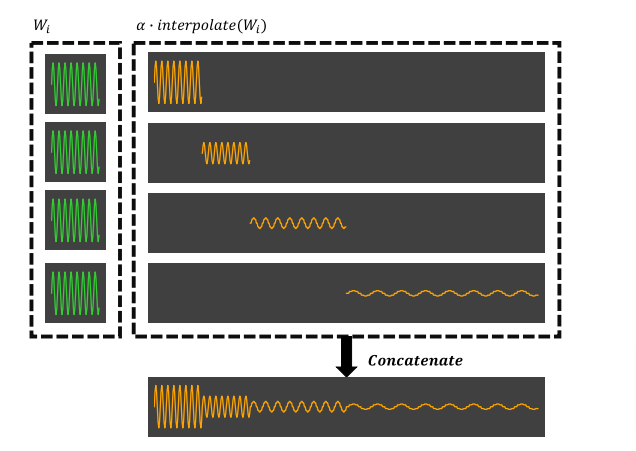
\includegraphics[width=0.4\textwidth]{Figs/sgconv.png}
        \label{fig:my_label}
    \end{figure}

    \begin{figure}
        \centering
        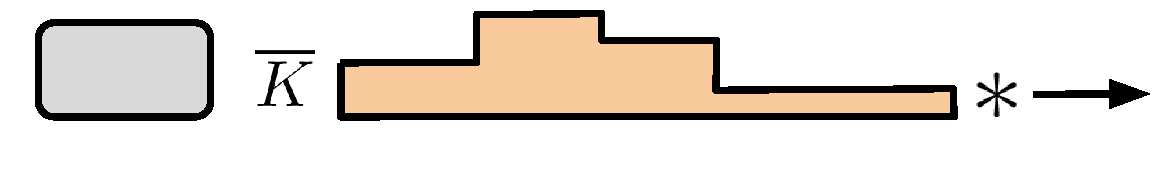
\includegraphics[width=0.5\textwidth]{Figs/SGParam.pdf}
        \label{fig:my_label}
    \end{figure}

\pause
    \begin{center}
    \alert{However}, no linear RNN form.        
    \end{center}
    
\end{frame}



\begin{frame}{RNN Param: LRU \cite{Orvieto2023-an}}
    Stable diagonal parameterization of Linear RNN
    \begin{align*}
    \textcolor{green}{\bar{A}}_{j,j} &= \exp(-\exp({\nu_j}) + i \exp(\theta_j))\\
    \textcolor{blue}{\bar{B}}_{j} &= (1 - |\bar{A}_{j,j}|^2)^{1/2}
    \end{align*}

    \begin{figure}
        \centering
        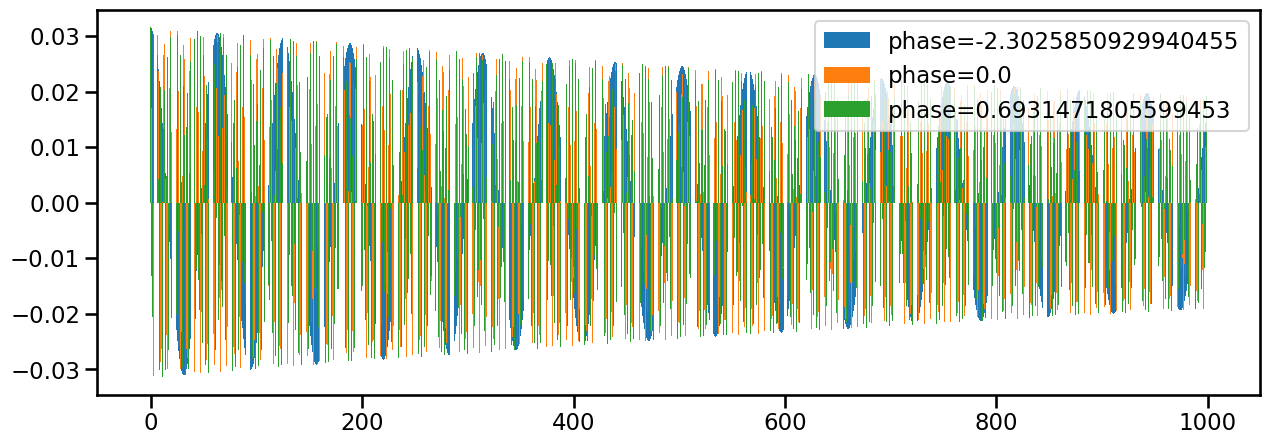
\includegraphics[width=0.8\textwidth]{Figs/phase.png}
        \label{fig:my_label}
    \end{figure}
\end{frame}

\begin{frame}{RNN Param: MEGA \cite{ma2022mega}}
     Use a parameterized damped, exponential moving average
    \begin{align*}
    \textcolor{green}{\bar{A}}_{j,j} &= 1 − \alert{\alpha_j} \times \delta_j \\
    \textcolor{blue}{\bar{B}}_{j} &= \alpha_j
    \end{align*}
    \begin{figure}
        \centering
        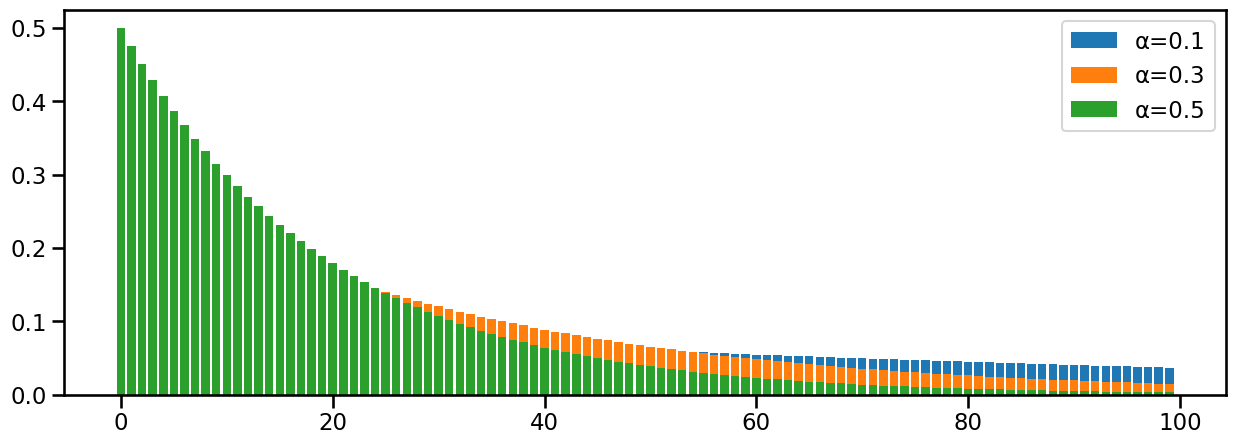
\includegraphics[width=0.7\textwidth]{Figs/ema.png}
        \label{fig:my_label}
    \end{figure}
    \begin{center}
    Very good results on NLP tasks like Translation. 
    \end{center}
    
\end{frame}


\begin{frame}{RNN Param: RWKV \cite{Peng2023-yp}}
    Inspired by Attention 
    
    Split into Keys, Values, and Receptance (no Query):
    \begin{align*}
    K_i, V_i, R_i
    \end{align*}
    \pause 
    Then compute averaged values normalized by keys. 
    
    \begin{align*}
     R_i\frac{\sum_{i'=1}^i \textcolor{green}{\exp(w)}^{i'}\exp(K_{i'}) V_{i'}} {\sum_{i'=1}^i \textcolor{green}{\exp(w)}^{i'}\exp(K_{i'})\phantom{ V_{i'}}} = R_i \frac{\text{LR}_1(\exp(K_i)V_i)}{\text{LR}_2(\exp(K_i))\phantom{V_i}}\\
    \end{align*}

    Yields a product of Linear RNNs (Computed directly).
    
\end{frame}


\begin{frame}{Results: RWKV \cite{Peng2023-yp}}
    \begin{center}
        Largest RNN. Trained up to 14B parameter scale.
    \end{center}
    \pause 
    \begin{figure}
        \centering
        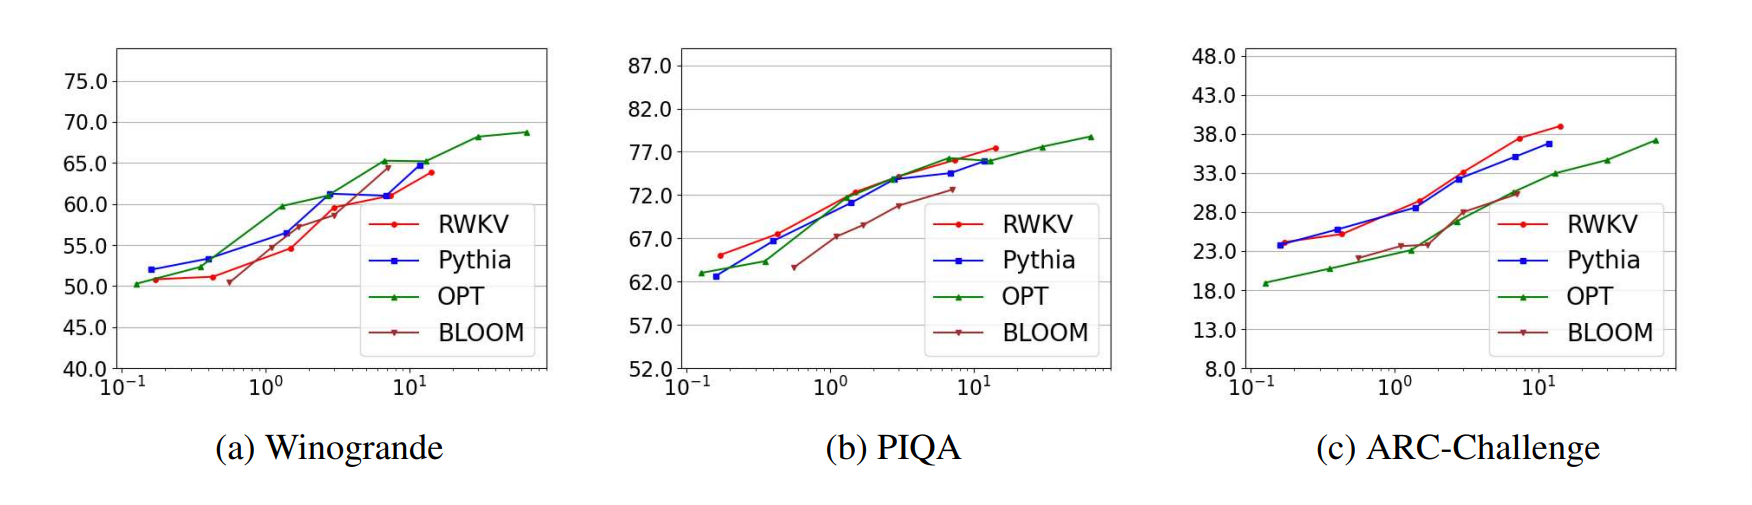
\includegraphics[width=1\textwidth]{Figs/RWKV.png}
        \label{fig:my_label}
    \end{figure}
    Lots of practical interest and community.
\end{frame}


\begin{frame}{Open Question: In-Context Learning}
    \begin{itemize}
        \item Results show comparable loss at medium scales.
        \item Significant interest is in abilities such as in-context learning
        \item Current understanding relies of Attention mechanisms.
    \end{itemize}
\end{frame}


% \begin{frame}{Parameterization: Diagonal RNN \cite{Li2022-pn}}
%     \begin{figure}
%         \centering
%         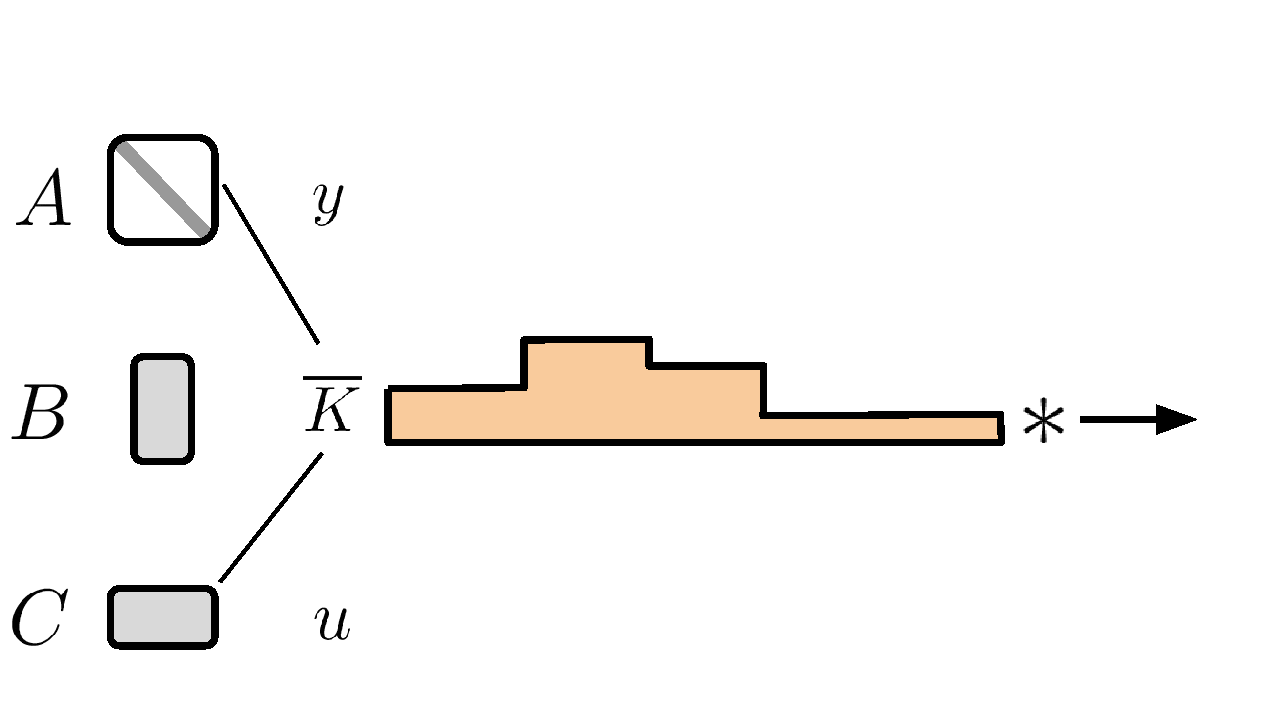
\includegraphics[width=0.5\textwidth]{Figs/DSSM.pdf}

%         \label{fig:my_label}
%     \end{figure}
% \end{frame}

% \begin{frame}{Results: GSS   $\downarrow$}
%         \begin{figure}
%         \centering
%         \includegraphics[width=0.7\textwidth]{}
%         \caption{Caption}
%         \label{fig:my_label}
%     \end{figure}
% \end{frame}





% \begin{frame}{Results: MEGA \cite{ma2022mega} $\uparrow$}
%     \begin{figure}
%         \centering
%         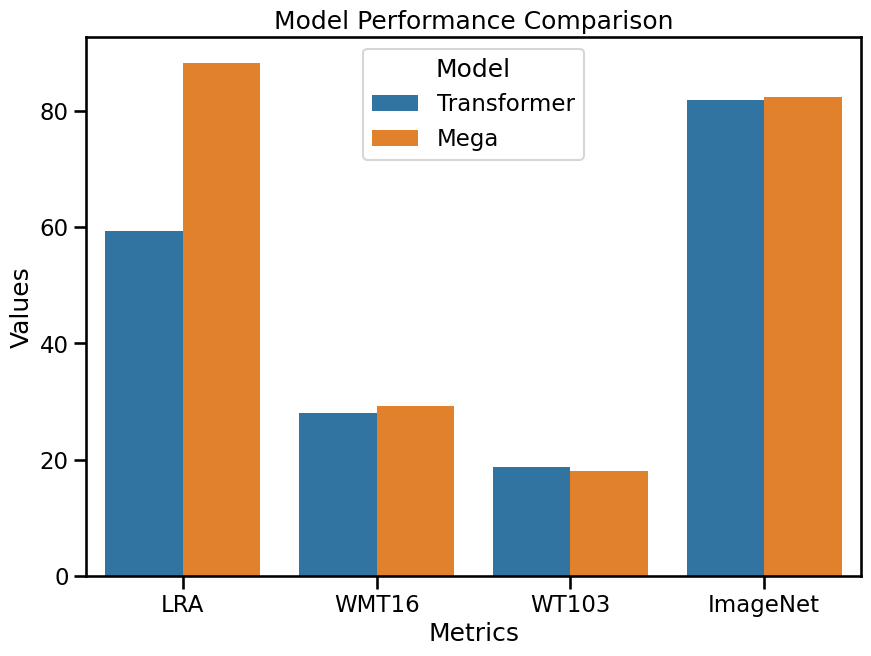
\includegraphics[width=0.7\textwidth]{Figs/Mega.png}
%         \label{fig:my_label}
%     \end{figure}
% \end{frame}


% \section{Computation and Parameterization}
% 
% \begin{frame}{Usage}

%     Linear RNNs opens up the modeling design space

%     \vspace{1cm}
%     \begin{itemize}
%         \item How to efficiently calculate?
%         \item How to parameterize?
%     \end{itemize}
% \end{frame}

% \begin{frame}{Calculation}
%     Recall the main calculation is a $L$ length convolution, 
    
%     \begin{figure}
%         \centering
%         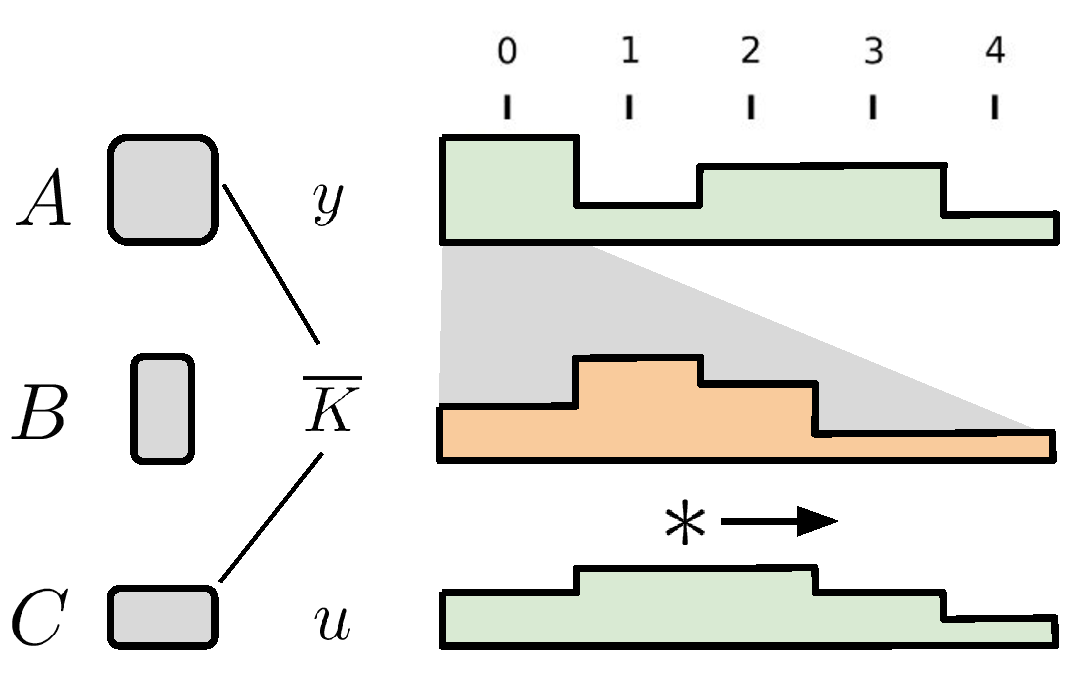
\includegraphics[width=0.7\textwidth]{Figs/SSM.pdf}
%         \label{fig:my_label}
%     \end{figure}
% \end{frame}



\begin{frame}{Method 2: Parallel Associative Scan \cite{smith2022simplified} }
    Compute $e_1\bullet \ldots \bullet e_l$ for any associative operator $\bullet$

\begin{center}
\Tree [.$\bullet$ [.$\bullet$ [.$\bullet$ $e_1$ ] [.$\bullet$ $e_2$ ] ] [.$\bullet$ [.$\bullet$ $e_3$ ] [.$\bullet$ $e_4$ ] ] ]
    
\end{center}
    \cite{Blelloch1990-yo,Martin2018-bq}
\end{frame}

\begin{frame}{}
    \[e_k = (\boldsymbol{E}_k, \boldsymbol{e}_k) = (\bar{\textcolor{green}{\boldsymbol{A}}}, \bar{\textcolor{blue}{\boldsymbol{B}}}u_k)\]
    \begin{figure}
        \centering
        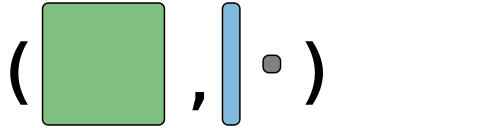
\includegraphics[height=0.1\textwidth,clip,trim={0cm 0cm 5cm 0cm}]{Figs/assoc.png}
        \label{fig:my_label}
    \end{figure}

    \[e_i \bullet e_j = (\boldsymbol{E}_i \boldsymbol{E}_j, \boldsymbol{E}_j \boldsymbol{e}_i + \boldsymbol{e}_j ) \]
    \begin{figure}
        \centering
        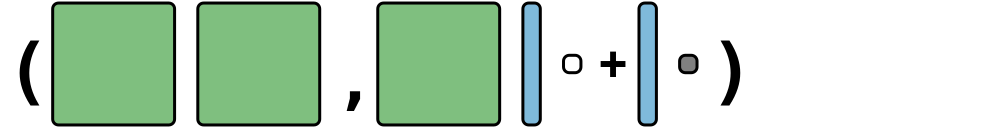
\includegraphics[height=0.1\textwidth,clip,trim={0cm 0cm 6cm 0cm}]{Figs/assoc2.png}
    \end{figure}
\end{frame}



% \begin{frame}{Parmeterization of RNN Models}
%     SSM framing gives an elegant parameterization of Linear RNNs,

%     \begin{figure}
%         \centering
%         \includegraphics[width=0.7\textwidth]{Figs/SSMParam.pdf}
%         \label{fig:my_label}
%     \end{figure}

%     Researchers have explored other parameterizations
% \end{frame}














\section{Scaling Linear RNNs}


\begin{frame}{Benefits of Linear RNNs}
    \begin{itemize}
        \item Methods for training (CNN) and generation (RNN)
        \item Potentially more FLOP efficient. 
        \item However not yet used in practice 
    \end{itemize}    
\end{frame}

\begin{frame}[c]{Current Efficiency with Scale \cite{Poli2023-ag}}
\begin{figure}
    \centering
    \includegraphics[width=\textwidth]{Figs/hyena.png}
    \caption{}
\end{figure}
 Models become more efficient at long time-scales.
\end{frame}

\begin{frame}{Issues on Accelerators}
    Approaches require:
    \vspace{0.5cm}

    \begin{itemize}
        \item Support for complex numbers
        \item Support for FFT (lower precision, TPU)
        \item Numerical Stability
        \item Fast Associative Scans 
    \end{itemize}
    \vspace{0.5cm}
    
    Hard to compete with pure MatMul in Attention.
\end{frame}

\begin{frame}{}
    \begin{figure}
        \centering
        \includegraphics[width=0.7\linewidth,clip,  trim={0.1cm 0.1cm 0.1cm 0.1cm}]{Figs/Is-Attention-All-You-Need-.png}
        \label{fig:my_label}
    \end{figure}
\end{frame}


% \begin{frame}{Frame Title}
%     Call to action. 

%     * Modeling benefits
%     * Theoretical approaches
%     * interplay with hardware efficiency. 
%     * Matching transformers 
%     * FFT / Complex 
%     * Associative scans
%     * GPU / TPUs 
%     * Models are more flop efficient, FLOPs are not equal. 
%     * Matmuls are more efficienct. 
%     * Numerical stability / complex numbers 
%     * 
% \end{frame}




% \begin{frame}{State Retrieval}
%     \begin{itemize}
%         \item Benchmarks compare perplexity of models
%         \item Significant interest is in abilities such as in-context learning
%         \item Current understanding relies of set-based Transformer mechanisms.
%     \end{itemize}
% \end{frame}




% \begin{frame}{In-Context Learning}
%     \begin{itemize}
%         \item Benchmarks compare perplexity of models
%         \item Significant interest is in abilities such as in-context learning
%         \item Current understanding relies of set-based Transformer mechanisms.
%     \end{itemize}
% \end{frame}

% \begin{frame}{Better Transformers}
%     \begin{itemize}
%         \item Models are being scaled to longer ranges (>100k)
%         \item For language, approximations of attention may be fine.
%         \item 
%     \end{itemize}
% \end{frame}


% \begin{frame}{Inductive Bias}
%     \begin{itemize}
%         \item Transformers are set-based models 
%         \item Linear RNNs encoder sequential bias
%         \item For language, unclear whether this is beneficial or not.
%     \end{itemize}
% \end{frame}


% \section{Practicalities}




% \begin{frame}{A slide title}

  \begin{itemize}
    \item A bulleted item
    \item Another item
      \begin{itemize}
        \item With sub-bullets
        \item And another, with some \textbf{bold} text
      \end{itemize}
    \item And another, at the top level, with \textit{italic} text
  \end{itemize}

  \note{
    Here's a note for this slide.
  }

\end{frame}

% \begin{frame}{A 50-50 split slide}

  \begin{columns}
    \begin{column}{0.5\linewidth}
      \begin{itemize}
        \item This side has a bullet
        \item And another bullet, with text that wraps if it's long
      \end{itemize}
    \end{column}
    \begin{column}{0.5\linewidth}
      \begin{figure}
        \centering
        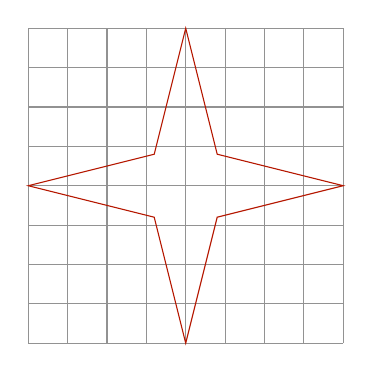
\begin{tikzpicture}[scale=2]
          \draw[step=0.25cm,color=gray] (-1,-1) grid (1,1);
          \draw[color=red] (1,0) -- (0.2,0.2) -- (0,1) -- (-0.2,0.2) -- (-1,0)
          -- (-0.2,-0.2) -- (0,-1) -- (0.2,-0.2) -- cycle;
        \end{tikzpicture}
        \caption{A figure caption}
      \end{figure}
    \end{column}
  \end{columns}

  \note{
    This slide has notes too.
  }

\end{frame}

% \begin{frame}{Full-slide figure}

  \begin{figure}
    \centering
    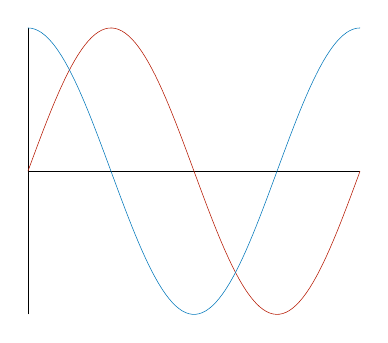
\begin{tikzpicture}[scale=0.5]
      \begin{axis}[
          scale only axis,
          no markers,
          domain=0:2*pi,
          samples=100,
          axis lines=center,
          axis line style={-},
          ticks=none]
        \addplot[red] {sin(deg(x))};
        \addplot[blue] {cos(deg(x))};
      \end{axis}
    \end{tikzpicture}
  \end{figure}
    \blfootnote{[Here is a citation]}


\end{frame}

% \begin{frame}{A slide with centered text}

  \begin{center}
    Some statement that is centered.
  \end{center}

  \vspace{2ex}
  \begin{center}
    \scriptsize (a small note)
  \end{center}

\end{frame}

% \begin{frame}[fragile]{A slide with some code}

	\begin{columns}
		\begin{column}{0.5\linewidth}
			\footnotesize
			\begin{Verbatim}[commandchars=\\\{\}]
/* some code */
def foo(x):
  return x**0.5 + 2*x

\color{blue}/* some can be highlighted */
\color{blue}foo(3)
      \end{Verbatim}
    \end{column}
    \begin{column}{0.5\linewidth}
      {\color{red} Some explanatory text, in red, with some \texttt{monospace} text.}
      There might be some math, too:

      $$\sqrt{x} + 2x$$
    \end{column}
  \end{columns}

\end{frame}

% \begin{frame}{A slide with some bracketed text}

	\begin{itemize}
		\item Some statement {\color{gray} [Some citation]}
		\item Another statement {\color{gray} [Another citation]}
		\item A final statement {\color{gray} [The last citation]}
	\end{itemize}

	\vspace{3ex}
	\begin{center}
		\scriptsize (a small note)
	\end{center}

\end{frame}


% \begin{frame}{A slide with some text and a link}

  \begin{itemize}
    \item This slide has some text along with a link
      \begin{itemize}
        \item \textbf{Some bold text}: followed by an explanation
        \item \textbf{More bold text}: followed by more text
      \end{itemize}
    \item Another bullet, with sub-bullets
      \begin{itemize}
        \item A sub-bullet
        \item Another sub-bullet, with more text
      \end{itemize}
  \end{itemize}

  \vspace{2ex}
  \begin{center}
    \color{blue} \href{https://github.com/anishathalye/auriga}{github.com/anishathalye/auriga}
  \end{center}

\end{frame}

\begin{frame}[allowframebreaks]
        \frametitle{References}
        \footnotesize
        \bibliographystyle{apalike}
        \bibliography{ssm.bib,anthology.bib}
\end{frame}
\end{document}
